\documentclass{article}
\usepackage[utf8]{inputenc}
\usepackage{natbib}
\usepackage{graphicx}
\usepackage{caption}
\usepackage{subcaption}
%\usepackage{xcolor}
\usepackage[utf8]{inputenc}
\usepackage[english]{babel}
\usepackage[dvipsnames]{xcolor}
\usepackage{multirow}
\usepackage{array}
\usepackage{wrapfig}
\usepackage{tabularx}
\usepackage{enumitem}
\usepackage{rotating}
\usepackage{appendix}
\usepackage{amsmath}
\usepackage{calc}
\usepackage[section]{placeins}

\setcitestyle{square}

\title{Electronics and Computer Science \\ Faculty of Physical Sciences and Engineering \\ University of Southampton \bigskip \bigskip \bigskip \bigskip \bigskip \bigskip \bigskip\\ Fedor Selenskiy \\ May 2020 \bigskip \bigskip \bigskip \bigskip \bigskip \bigskip \bigskip \\ Use of Machine Learning to Improve Eating Habits \bigskip \bigskip \bigskip \bigskip \bigskip \bigskip \bigskip\\ Project supervisor: Dr Heather Packer \\ Second examiner: Dr Paolo Rapisarda \\ A progress report submitted for the award of
BSc Computer Science}
\bigskip
\bigskip
\bigskip
\bigskip
\date{}

\begin{document}
\maketitle
\newpage

\newpage
\section{Abstract}
In this project, I created a cloud based Android application that estimates a user's Healthy Eating Index score and uses machine learning techniques to recommend healthy food items maximising their HEI score, that the user is likely to enjoy. 

\newpage
\section{Statement of Originality}
\bigskip
\begin{itemize}
    \item I have read and understood the ECS Academic Integrity information and the University’s
    Academic Integrity Guidance for Students.
    \item I am aware that failure to act in accordance with the Regulations Governing Academic Integrity
    may lead to the imposition of penalties which, for the most serious cases, may include
    termination of programme.
    \item I consent to the University copying and distributing any or all of my work in any form and
    using third parties (who may be based outside the EU/EEA) to verify whether my work
    contains plagiarised material, and for quality assurance purposes.
\end{itemize}
\bigskip

\begin{enumerate}
    \item I have acknowledged all sources, and identified any content taken from elsewhere.
    \item I have not used any resources produced by anyone else
    \item I did all the work myself, or with my allocated group, and have not helped anyone else.
    \item The material in the report is genuine, and I have included all my data/code/designs. 
    \item I have not submitted any part of this work for another assessment.
    \item My work did not involve human participants, their cells or data, or animals.
\end{enumerate}

\newpage
\section{Acknowledgements}
I would like to thank my supervisor, Dr Heather Packer, for guiding me through the project. I would also like to thank my father, Dr Evgeny Selensky, for insightful comments on the technical aspect of the project, and my older brother, Nick Selensky, for helpful comments regarding the user interface of the application.

\newpage
\tableofcontents

\newpage
\section{Acronyms}
\begin{itemize}
    \item \textbf{EM}: Expectation Maximisation
    \item \textbf{UI}: User Interface
    \item \textbf{API}: Application Programming Interface
    \item \textbf{DAO}: Data Access Object
    \item \textbf{DGA}: Dietary Guidelines for Americans
    \item \textbf{GMM}: Gaussian Mixture Model
    \item \textbf{HEI}: Healthy Eating Index
    \item \textbf{URI}: Universal Resource Identifier
    \item \textbf{URL}: Universal Resources Locator
    \item \textbf{FPED}: Food Patterns Equivalents Database
    \item \textbf{REST}: Representational State Transfer
    \item \textbf{USDA}: United States Department of Agriculture
    \item \textbf{MVVM}: Model-View-ViewModel design architecture
    \item \textbf{JSON}: JavaScript Object Notation
    \item \textbf{HTTP}: Hypertext Transfer Protocol
    \item \textbf{HTTPS}: Hypertext Transfer Protocol Secure
    \item \textbf{WWEIA}: What We Eat In America
    \item \textbf{FNDDS}: Food and Nutrition Database for Dietary Studies
\end{itemize}

\newpage
\section{Introduction}
\subsection{Problem}
There exists a wide variety of health and fitness applications. A lot of the food tracking applications, such as MyFitnessPal, serve as food diaries and progress trackers. Such applications typically show the user the total amount of calories they consumed, as well as providing a nutritional breakdown of logged food items. This leaves the interpretation of the collected data to the user. 

\bigskip
\noindent A user with a lack of experience may struggle to effectively utilise such data. The user may begin to question whether they are eating too much or too little, whether they are eating the right foods, and whether their diet is actually healthy. I aim to create an Android application that will aid an individual in gaining a deeper understanding of the quality of their diet by estimating the Healthy Eating Index (HEI) of the set of foods consumed in a day, as well as make personalised recommendations on food items that will increase their HEI score.

\subsection{Goals}
This application should:
\begin{enumerate}
  \item Enable the user to keep a food diary, where the user inputs the food items they consumed.
  \item Estimate HEI based on the food input.
  \item Use a machine learning algorithm to build a recommender system that would suggest food items the user might like that will increase their HEI.
  \item Present the HEI score in a radar graph in order to help the user gain a better understanding of their diet.
\end{enumerate}

\subsection{Scope}
\noindent The datasets available to me are relatively small and not detailed. For example, portion sizes of the food items are required to calculate HEI. Such information was missing, thus assumptions and approximates had to be made. Similar techniques and methods could be applied to larger and more detailed datasets, which would eliminate the need for such approximations, and result in more accurate HEI estimates. Using a bigger dataset would result in more personalised recommendations.

\newpage
\section{Literature Review}
\subsection{Background Research}
\subsubsection{Healthy Eating Index}
Many people may not even be aware that they are consuming too much or too little of a specific food category, as they may not be aware of the dietary guidelines. This may lead to undesirable effects, for example not eating enough fruits and vegetables may lead to vitamin deficiency, or excessive consumption of added sugars can lead to weight gain. Easy access to the HEI score of an individual may help raise awareness of their consumption of certain food groups, and hopefully encourage them to become healthier. 
\bigskip

\noindent HEI \cite{hei_2015} is a density-based measure for assessing the dietary quality by measuring the degree to which a set of foods aligns with the Dietary Guidelines for Americans (DGA). Food items are scored based on the pertinent densities of its constituents, which fall into one of 13 categories, referred to here as HEI components. 

\bigskip
\noindent The average score of the 13 components represents the overall diet quality, while individual component scores can help reveal strengths weaknesses of the diet. HEI does not account for the amount of food consumed, as all components represent amounts per 1000 kcal (with the exception of Fatty Acid Ration component, which is a ratio). See Table \ref{table:hei_2015_table_adapted} for HEI 2015 scoring standard.

\begin{table}[h]
\hspace*{-1.7cm} 
\centering
\begin{tabular}{||c|m{5cm}|m{5cm}||}
\hline
    Component & Standard for Max Points & Standard for Min Points \\ [0.5ex] 
    \hline
    Total Fruit & $\geq$ 0.8 c equivalents (5 points) & No fruit\\
    \hline
    Whole Fruit & $\geq$ 0.4 c equivalents (5 points) & No whole fruit\\
    \hline
    Total Vegetables & $\geq$ 1.1 c equivalents (5 points) & No vegetables\\
    \hline
    Greens \& Beans & $\geq$ 0.2 c equivalents (5 points) & No dark green vegetables or legumes\\
    \hline
    Whole Grains & $\geq$ 1.5 c equivalents (10 points) & No whole grains\\
    \hline
    Dairy & $\geq$ 1.3 c equivalents (10 points) & No dairy\\
    \hline
    Total Protein Foods & $\geq$ 2.5 c equivalents (5 points) & No protein foods\\
    \hline
    Seafood \& plant proteins & $\geq$ 0.8 c equivalents (5 points) & No seafood or plant proteins\\
    \hline
    Fatty Acid Ratio \dagger & (PUFAs + MUFAs)/SFAs $\geq$ 2.5 (10 points) & (PUFAs + MUFAs)/SFAs $\leq$ 1.2\\
    \hline
    Refined Grains & $\leq$ 1.8 oz equivalents (10 points) & $\geq$ 4.3 oz equivalents\\
    \hline 
    Sodium & $\leq$ 1.1 gram (10 points) & $\geq$ 2.0 grams\\
    \hline 
    Added Sugars & $\leq$ 6.5\% of energy (10 points) & $\geq$ 26\% of energy\\
    \hline
    Saturated Fats & $\leq$ 8\% of energy (10 points) & $\geq$ 16\% of energy\\
\hline
\end{tabular}
\caption{Scoring Standards for HEI 2015 (adapted from source \cite{hei_2015})}
\label{table:hei_2015_table_adapted}
\end{table}

\noindent $\dagger$ Polyunsaturated Fatty Acids (PUFA), Monounsaturated Fatty Acids (MUFA), Saturated Fatty Acids (SFA).

\noindent The basics steps in calculating HEI are: 

\begin{enumerate}
    \item Acquiring a set of foods to consider.
    \item Determining the total amount of each dietary constituent across the set.
    \item Deriving pertinent densities of each dietary constituent and scoring against the HEI standard.
\end{enumerate}

\subsubsection{Side Effect of Diets}
Diets focusing on macronutrient intake may affect the micronutrient intake of an individual. A study on the micronutrient quality of weight-loss diets \cite{micro_quality} has shown that a significant proportion of the participants following the Ornish diet have shifted to intakes associated with risk of inadequacy of vitamin E and B-12 and zinc. On the other hand, the risk of inadequacy of vitamins A, E, K and C was found to decrease in participants following the Zone diet. 

\subsubsection{Satiety and Satiation}
A study on the relationship between regular eating adherence and binge eating frequency \cite{binge_freq} shows that a higher number of regular eating adherent days is has a high positive correlation with lower binge eating frequency. This provides evidence to suggest that regular satiety and satiation can reduce food craving.
\bigskip

\noindent Many factors can influence satiation, which ends a meal, and satiety, which determines the time between meals. Macronutrient intake plays an important role in both satiation and satiety. Protein is the most effective macronutrient in prolonging the feeling of fullness \cite{satiety_satiation}. Additionally, an increase in protein consumption has been shown to increase diet-induced thermogenesis \cite{satiety_satiation}, which contributes to 10\% of daily energy expenditure \cite{weight_expenditure}.
\bigskip

\noindent Food volume contributes to satiation more than energy content. Therefore reducing the energy density of the food, or consumption of food with a lower energy density, is a way to promote satiation \cite{satiety_satiation}. 
 \bigskip

\newpage
\subsubsection{Food Craving}
Modern temptations to eat are stronger than in the past \cite{tempted_brain}. Despite many efforts to increase health awareness, from social media influence to regulations on food labelling  \cite{food_label}, we still fall victim to craving junk food. 
\bigskip

\noindent Different environmental factors can affect food craving. A study on the effects of the time of day on momentary hunger and food craving \cite{craving_time} has shown that there is a high coherence between hunger and craving, and that desirability of a food group is affected by the time of day. An individual's mood or exposure to food-related cues are potentially the biggest triggers of craving \cite{craving_sweets}, which means that it may prove difficult for an individual to be rid of cravings completely. 
\bigskip

\noindent In extreme cases, food craving could be the result of brain reward circuit dysfunction. That may be so if the motivation for food consumption begins to occur without hedonic liking of the food, which are usually connected processes \cite{tempted_brain}. Conversely, reward circuit dysfunction could be the result of excessive food consumption. More of the pleasurable food has to be consumed to trigger the same level of reward circuit activation, which has built up a tolerance due to overeating \cite{tempted_brain}.
\bigskip

\subsubsection{Summary of Background Research}
Understanding the cause of food craving is important in overcoming it. Suggesting to reduce the time between meals to an individual to reduce hunger could also help them reduce cravings. Conversely, suggesting a planned cheat meal to an individual with cravings could activate the brain reward circuits, thus satisfying the cravings. Estimating the HEI scores of the individual categories can clarify what foods categories the user is scoring less in. Foods from those categories maximising satiation and satiety can then be suggested. 

\subsection{Technical Research} 
\subsubsection{Android Application Overview}
Android applications are built from the following components which are entry points through which the system or the user can enter the application \cite{android_fundamentals}:

\begin{itemize}
    \item \textbf{Activity}: entry point for the user which contains the user interface.
    \item \textbf{Service}: entry point for running the application in the background, which does not require a user interface.
    \item \textbf{Broadcast receiver}: component enabling the event delivery to the application outside of use, and reception of broadcast announcements. 
    \item \textbf{Content provider}: manages application data and its accessibility by other applications. 
\end{itemize}

\bigskip 
\noindent The main building blocks of an Android application include the following: 

\begin{itemize}
    \item \textbf{View}: represents a visual component in the application \cite{android_view}. All visual components extend this class. In order for the user to be able to interact with a View, it must implement event handling and drawing. 
    \item \textbf{Fragment}: represents a collection of related Views \cite{android_fragment}. Combination of Fragments can be used to construct a dynamic UI inside an Activity. 
    \item \textbf{ViewModel}: serves as an abstraction layer between the Activities or Fragments and the data \cite{android_view_model}, also storing UI data. In order to ensure high cohesion and low coupling, communication amongst Fragments and between Fragments and Activities is achieved via the ViewModel \cite{android_app_architecture}
    \item \textbf{LiveData}: life-cycle aware, observable data holder class \cite{android_live_data}. A LiveData object can be observed for changes, and those changes can be acted upon accordingly. Life-cycle awareness ensures that when the data changes, only active observers are notified.
    \item \textbf{Room Persistence Library}: architectural components serving as an abstraction layer over SQLite \cite{android_room}. An Entity class describes the structure of a table in a RoomDatabase class. A DAO interface defines the SQLite queries that Room uses to automatically generate Entity objects, which represent specific entries in the table. Values can be accessed with defined getter methods from the Entity object.
\end{itemize}

\subsubsection{Android Application Architecture}
Android applications are not required to adhere to a specific architecture. However, a good design architecture could boost development time, improve the maintainability, extensibility, and performance of the application \cite{passive_mvc}. 

\bigskip
\noindent Android developers at Google advise to decouple the UI from the data by using a Model-View-Viewmodel (MVVM) \cite{mvvm} architecture when writing an Android application \cite{android_app_architecture}. MVVM  architectural components serve the following purpose: 

\begin{itemize}
    \item \textbf{Model}: representation of the data. Room persistence library \cite{android_room} is an example of Model representation in Android.
    \item \textbf{View}: all the visual components, what the user actually sees. This is represented by classes such as View, Activity and Fragment. 
    \item \textbf{Viewmodel}: intermediary between the raw data and the view, acting as a layer of abstraction. This allows the view to be developed independently of the model. ViewModel class in Android is an implementation of this structure. 
\end{itemize}

\bigskip
\noindent Separation of the view from the model helps maintain good user experience, by minimising the workload of the view. This is especially important for low powered devices running Android. 

\subsubsection{Machine Learning Algorithms}
Machine learning is a subset of artificial intelligence that can learn patterns from data without having to define them a priori. Categories of machine learning algorithms include \cite{ml_enterprises}:

\begin{itemize}
  \item \textbf{Supervised machine learning} is used to discover mapping function for input and corresponding output dataset, which can be used for decision making, such as prediction and classification (putting data in predefined classes).
  \item \textbf{Unsupervised machine learning} is used to capture the relationship, or the correlation, among input data, which can be used for clustering (the process of grouping similar data with no predefined classes).
  \item \textbf{Semisupervised machine learning} is a multistage process in which one learning type is used as preprocessing for the other.
  \item \textbf{Reinforcement learning} algorithms learn behaviour based on reward mechanisms.
\end{itemize}

\noindent The data available to me limits me to the use of unsupervised machine learning algorithms, as the MyFitnessPal dataset \cite{diet_success_predictions} I am going to be working with contains practically raw data with minimal processing.

\bigskip
\noindent K-Means clustering is an unsupervised machine learning algorithm which aims to group data points into 'k' clusters, where the value of 'k' is defined \textit{a priori} \cite{k_means}. This iterative process is initialised by randomly generating 'k' data points, which are called centroids. At every consecutive iteration, every data point is assigned to the closest centroid. The mean value of all the data points assigned to a centroid is calculated, and the centroid is shifted to that mean position. This process is repeated until the centroids stop shifting between iterations. K-Means is fast as it has linear time complexity, but fails when clusters are not circular or their means are close together, which is a result of using the mean as a cluster centre.

\bigskip
\noindent Expectation Maximisation (EM) is a more general approach \cite{k_means}. EM algorithms aim to find parameters to statistical models of clusters in a way that maximises the likelihood of data points belonging to those clusters. EM algorithms allow different assumptions about the shapes of the clusters to be made. Similarly to K-Means, the number of clusters has to be chosen \textit{a priori}, and the parameters of each cluster are chosen randomly. Each iteration consists of two steps. The first 'E' step generates the expectation function for each cluster. The second 'M' step finds parameters that maximise the expectation \cite{expectation_maximisation}. Gaussian Mixture Model (GMM) is a statistical model where the data is assumed to be derived from multiple normal distributions \cite{gmm}. Modelling data with GMM and using an EM algorithm can be used to cluster data. GMM offers greater flexibility in the shape of the clusters, and supports mixed membership. 

\subsubsection{Cloud Computing}
\textit{'Cloud computing is a model for enabling convenient, on-demand network access to a shared pool of configurable computing resources (e.g., networks, servers, storage, applications, and services) that can be rapidly provisioned and released with minimal management effort or service provider interaction.'} \cite{cloud_computing}
\bigskip

\noindent Important components of cloud computing include \cite{cloud_computing}:

\begin{itemize}
    \item On-demand self-service: consumers can gain access to resources automatically.
    \item Network access: computing resources are accessed through the internet.
    \item Resource pooling: computing resources are assigned to users based on demand
\end{itemize}

\subsubsection{HTTP}
HTTP is a stateless application layer protocol used for communication over the World Wide Web. Stateless means that every HTTP request must be complete and not use any state information. An HTTP URL consists of three main parts. For example \textit{”http://example.com:80/dir1/dir2/file?a=1b=2”}:

\begin{itemize}
    \item \textbf{Host}: example.com:80 points to a host located at the IP address associated with example.com on port 80.
    \item \textbf{Path}: the requested resource is located in the path ”/dir1/dir2/file”.
    \item \textbf{Query}: the query, separated from the path by a question mark, contains any required parameters separated by an ampersand.
\end{itemize}

\bigskip
\noindent The two fundamental HTTP requests are GET and POST, both of which are used to retrieve data.  The key difference between the two is that GET puts the query parameters in the URL, whereas POST places the query parameters in the message body. However, it is  important  to  mention  that  neither  GET  nor  POST  HTTP  requests  are secure.  HTTPS should be used for secure communication as it uses encryption. 

\bigskip 
\noindent Offloading computationally intensive tasks, such as HEI calculations and generation of recommendations, to a server would make the Android application as fast and as lightweight as possible. The server would act as the cloud, by providing computing resources and remote storage capabilities. HTTP protocol would mediate the communication between the cloud and the Android application, with GET and POST requests being used 

\subsubsection{String Comparison Metrics}
String matching algorithms are designed to find a target string in a source document. Identifying food items in the user input would require an implementation of a string matching algorithm. A string comparison metric is required to evaluate the similarity of two strings in order to do string matching. String similarity metrics I am going to be using in this project are: 

\begin{itemize}
    \item \textbf{Levenshtein distance}: otherwise known as edit distance, this metric describes the smallest amount of edit operations required to transform one string into another \cite{levenshtein_distance}. An edit operation is the insertion, deletion or substitution of a single character. 
    \item \textbf{Jaccard index}: otherwise known as intersection over union, this metric describes the similarity of two sets. It is calculated by computing the number of elements in the intersection of two sets divided by the size of the union of those two sets. This could be very useful for comparing the similarity of sentences rather than just individual words, however this would still require a way of comparing individual words \cite{jaccard} \cite{string_similarity_ontology}. Given sets of words A and B, the Jaccard index of A and B is the following: 
    \begin{align*}
        Jaccard(A,B) &= \frac{A \cap B}{A \cup B}
    \end{align*}
\end{itemize}

\subsubsection{String Matching}
Wagner-Fischer algorithm computes the Levenshtein distance between two strings. It has time and space complexity of O(nm), where 'n' and 'm' are the lengths of the strings being compared \cite{wagner_fischer}. This algorithm is sensitive to word order, however it is straightforward to implement and to use, as strings with a lower edit distance are more likely to be a match than those with a higher edit distance. 

\bigskip
\noindent Jaccard index of two strings can be used in string matching. The similarity of words could be measured using an edit distance algorithm, such as Wagner-Fischer, and words could be considered similar if their edit distance is below a certain threshold. The number of similar words can then be divided by the size of the set of words in both strings.

\bigskip
\noindent Mongue-Elkan algorithm is used to match sentences by computing the average similarity of closest words from each string, giving it time complexity of O(nm), where 'n' and 'm' are the number of words in each string \cite{mongue_elkan}. This algorithm also requires the use of a similarity metric for determining closest word pairs. 

\bigskip
\noindent By definition, this algorithm is less sensitive to word order, thus making it more desirable for real-world applications. Given a similarity metric 'sim' and sets of words A,B, Mongue-Elkan measure is the following \cite{mongue_elkan}: 

\begin{align*}
    Mongue-Elkan(A,B) &= \frac{1}{|A|} \sum_{i=1}^{|A|} max\{sim(a_i,b_j)\}_{j=1}^{|B|}
\end{align*}

\noindent Sergio Jimenez et. al. \cite{mongue_elkan} propose a modification to the Mongue-Elkan algorithm that will promote words with higher similarity, as they are assumed to be more informative, using generalised mean:

\begin{align*}
    Generalised Mongue-Elkan(A,B) &= (\frac{1}{|A|} \sum_{i=1}^{|A|} (max\{sim(a_i,b_j)\}_{j=1}^{|B|})^m)^{\frac{1}{m}}
\end{align*}

\noindent The value of 'm' represents the degree to which higher similarity words are prioritised. 

\subsubsection{Recommender Systems}
A recommender system is a personalised information filtering system for providing useful item suggestions \cite{recommender_systems_handbook}. Types of recommender systems include: 

\begin{itemize}
    \item \textbf{Content based}: this type of recommender system aims to suggest items with similar features to items that the user previously liked. 
    \item \textbf{Knowledge-based}: this type of recommender system utilises domain knowledge to suggest items with features that would meet the user's needs.
    \item \textbf{Collaborative filtering}: this type of recommender system suggests items that similar users liked in the past.
    \item \textbf{Hybrid}: this type of recommender system uses a combination of techniques.
\end{itemize}

\bigskip
\noindent With the currently available to me resources, it is incredibly difficult to build a content or knowledge-based recommender system. Luckily, the nature of the MyFitnessPal dataset \cite{diet_success_predictions} would make it possible to build user models for 9'800 real-world users. As a result, a collaborative filtering recommender system would be the most suitable. 

\bigskip
\noindent My approach is to generate feature vectors that represent users, and group users by clustering their corresponding feature vectors using a clustering algorithm. The clusters will contain groups of users with similar diets, who are therefore likely have similar food tastes. Based on this implicit collaborative filtering, a set of foods that any particular user is likely to find enjoyable can be generated by looking at what other users from the same cluster have consumed in the past. Foods with the highest HEI score can then used as recommendations for the user of interest.

\bigskip
\noindent Unsupervised machine learning algorithms are the most suitable for the available datasets, which contain practically raw data. In order to make the recommender system fast, an algorithm with a fast time complexity is desirable. 
However, scalability may be an issue. 

\bigskip
\noindent I talked about K-Means clustering algorithm in section 5.2.3 'Machine Learning Algorithms', mentioning the fact that it has linear time complexity. The problem with K-Means is that it has to be rerun with every new user. A user with a drastically different diet may upset the existing clusters, which could lead to worse recommendations being produced. I believe that K-Means suffices for demonstrative purposes of this project, however the recommender system would have to be reevaluated if it were to be built with scalability in mind. 


\subsubsection{Summary of Technical Research}
Although there are no restrictions on the architecture of Android applications, a good design architecture can be very beneficial. Although it is advised to use MVVM architecture when building an Android application, some of the features of the Android Passive MVC \cite{passive_mvc} can be implemented to improve the application. For example, MVVM doesn't restrict Activities being made very bloated. Applying the general approach of the Android Passive MVC design by making the Activities and Fragments lightweight would definitely add to the user experience and fluidity of the UI. The application could be made even more lightweight by offloading the computationally intensive tasks to the cloud, providing a smooth and responsive experience to the end-user. 


\section{Proposed Final Design}
\subsection{Overview}
This project is the implementation of a cloud-based Android application that estimates a user's HEI. The application will serve as a food diary for gathering the necessary information to calculate the HEI estimate. 

\bigskip
\noindent A collaborative filtering recommender system will be used to suggest food items that the user may like in order to increase their HEI. MyFitnessPal dataset \cite{diet_success_predictions}, which contains food diaries of over 9000 users from 2014 to 2015, will be used to populate the recommender system. A user profile is going to be built for every user in the dataset, and a clustering algorithm will be used to group users with similar diets. 

\bigskip
\noindent The application is going to be written for Android in Java, following the advised MVVM architecture. The cloud-based component is going to be used for the storage of the user information and running the recommender system. Additionally, this approach provides privacy, as the end-user does not have access to other user's information. 

\newpage
\subsection{Justification}
\subsubsection{Cloud}
The reasons for implementing this project as a cloud application are as follows:
\begin{itemize}
    \item Running machine learning algorithms may be computationally intensive, offloading the task to the cloud would speed up the application.
    \item The model can be dynamically updated with every new user that joins and every new food diary entry.
    \item The user would have the option to retrieve their data in case they lose it locally.
\end{itemize}

\subsubsection{Android}
The reasons for using MVVM architecture in the development of the application are as follows:
\begin{itemize}
    \item MVVM is UI driven. 
    \item The architecture ensures the extensibility and maintainability of the application, which simplifies updating the application in the future.
    \item Updating visual components can be done independently of the data, thus making it easier to update the application with the newest HEI standards. 
\end{itemize}

\subsubsection{Estimating HEI}
Estimating the user's HEI can give very beneficial insight into their eating patterns. The user can be informed which food categories they are scoring low in, and foods belonging to those categories can be suggested to the user in order to increase their HEI score. 

\subsubsection{Recommender System}
One of the biggest problems that people face when it comes to dieting or attempting to improve their health, is replacing foods that they like with foods that they do not. 

\bigskip
\noindent While it is incredibly difficult to quantify something as subjective as taste, data science can reveal underlying patterns in what foods people may or may not like. Recommender systems are constantly used to offer users products based on the subjective liking of other products, such as movies and music. 

\bigskip
\noindent A recommender system can help tackle this issue, by advising the user to eat foods that are healthier, yet the user is still likely to enjoy. The assumption is made that people with similar diets are likely to have similar tastes. There are many factors that play a role in a person's diet, which could be biological or environmental. Thus the assumption is made that the user's diet is representative of the food they like.

\subsection{Requirements}
Table \ref{table:project_requirements} shows the non-functional and functional requirements.

\begin{table}[h]
\hspace*{-1.5cm} 
\centering
\begin{tabular}{||c|c|c|m{7cm}||}
\hline
    Number & Type & Name & Description \\ [0.5ex] 
    \hline 
    1 & Non-functional & Simple design & The application should have a simple, minimal design that is easy to follow. \\
    \hline 
    2 & Non-functional & Fast & The application should be fast and smooth. \\
    \hline 
    3 & Functional & Platform & The application should be available on Android. \\
    \hline
    4 & Functional & Logging & The application should allow the user to log the food they consume. \\
    \hline 
    5 & Functional & HEI score & The application should estimate the HEI score of the user based on the logged foods. \\
    \hline 
    6 & Functional & Presentation & The application should present HEI estimate in a radar graph. \\
\hline
\end{tabular}
\caption{Requirements}
\label{table:project_requirements}
\end{table}

\subsection{Layout and User Interface}
Figure \ref{fig:food_diary} shows a reference design of the food diary section of the application, and Figure \ref{fig:summary} shows a reference design of the summary section, where the HEI score is presented in a radar graph. 


\begin{figure}[h]
\centering
\begin{subfigure}{.5\textwidth}
  \centering
  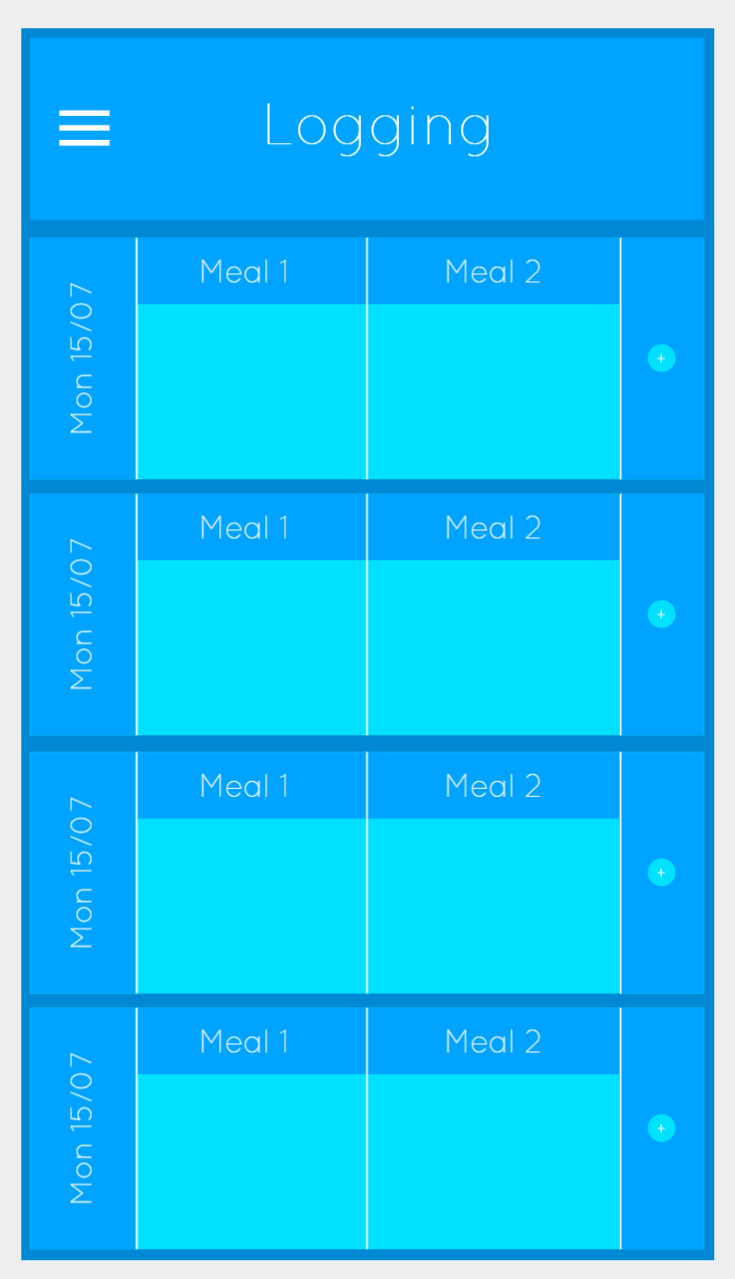
\includegraphics[width=3.8cm]{page1.jpg}
  \caption{Page 1: Food Diary}
  \label{fig:food_diary}
\end{subfigure}%
\begin{subfigure}{.5\textwidth}
  \centering
  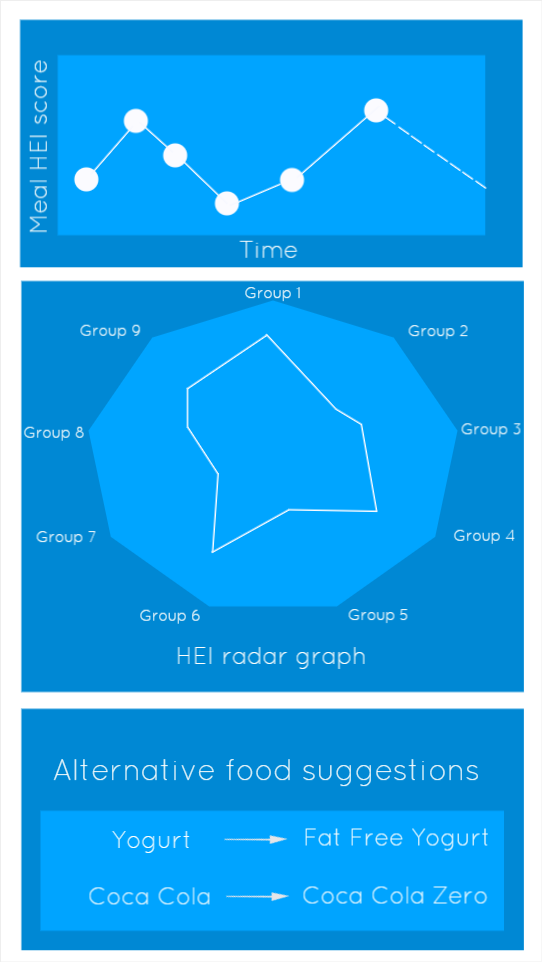
\includegraphics[width=3.8cm]{page_2_updated.png}
  \caption{Page 2: Summary}
  \label{fig:summary}
\end{subfigure}
\caption{Layout and User Interface Design of the Android Application}
\label{fig:reference_design}
\end{figure}

\section{Project Management}
\subsection{Project Planning}
Appendix D contains a Gantt chart with a breakdown of the work I planned to do at the beginning of the year 2020. Unfortunately, a few obstacles I ran into during the project really set me back. I successfully implemented the core functionality of the application as planned, but I did not manage to implement all of the additional features that I would have liked. 

\bigskip
\noindent I was originally planning on implementing sign up an log in functionality, where the users would sign up with an email, and log in upon email verification, as described in appendices A and C. 

\bigskip
\noindent There was a very steep learning curve in learning about Android application development.  I ran into a number of obstacles during the implementation of the Android application, including saving user input to internal memory and working with LiveData objects.
\bigskip

\subsection{Risk Assessment}
\begin{table}[h]
\centering
\hspace*{-1.3cm} 
\begin{tabular}{||c|c|c|c|c|m{6cm}||}
\hline
    Number & Risk & P & S & RI & Mitigation \\ [0.5ex] 
    \hline
    1 & Loss of work & 1 & 5 & 5 & Keep work online and keep backups in different locations. \\
    \hline
    2 & Small dataset & 3 & 3 & 9 & Look into identifying different eating patterns^\dagger. \\
    \hline
    3 & Erroneous application development & 3 & 3 & 9 & Regular code testing. Modularity of code could help ensure the development of one component will not affect the other components. \\ 
    \hline
    4 & Running out of time & 3 & 4 & 12 & Keep a structured working pattern. Make and adhere to a plan. Focus on producing a minimum viable product. Plan for slow progress by dedicating enough time for the project. \\
    \hline
    5 & Infeasibility of approach & 3 & 5 & 15 & Look into identifying different eating patterns^\dagger.  \\
    \hline 
    6 & Data not suitable & 3 & 5 & 15 & Search for datasets conveying different data. However, it could be possible that a suitable dataset is not publicly available. \\
    \hline
\end{tabular}
\caption{Risk assessment}
\label{table:risk_assessment}
\end{table}

\bigskip
\noindent Table \ref{table:risk_assessment} shows the risk assessment I carried out at the start of the year. P is the probability of the risk occurring on a scale of 1 to 5. S is the severity of the risk on a scale of 1 to 5. RI is the risk index of the risk, which is P*S. 

\bigskip
\noindent $\dagger$ Analysis of eating times, nutrient distributions throughout the day, or comparison of diets of users struggling to achieve a dietary goal with users who accomplished those goals could be done if calculations of HEI with the available resources are infeasible. 

\subsection{Encountered Problems}
During this project, I encountered risks 1,2,4 and 6 described in Table \ref{table:risk_assessment}. One global string matching technique I wanted to implement in addition to the others, was term frequency-inverse document frequency (TF-IDF) weighting for terms in the FNDDS database \cite{FNDDS}. I generated a table with the weights but erroneously deleted it, thinking it was an outdated table I no longer needed. 
\bigskip
\noindent The MyFitnessPal dataset \cite{diet_success_predictions} is relatively small, containing information on just under 10'000 users. One of the steps in building the recommender system, was to generate feature vectors for every user. I only had time to generate feature vectors for about 300 users, but that was sufficient to demonstrate the recommender system working.

\bigskip
\noindent The MyFitnessPal dataset was missing portion size, which is crucial in calculating HEI. I used the ratio of the number of calories in the user input to the number of calories in the matched food item from the FNDDS database to estimate portion size.

\bigskip
\noindent Calculating the HEI of a set of foods automatically is a very complex process. Matching food input to a food item in the FNDDS database allows making an estimate of the HEI score relatively quickly, using required precalculated information. The FNDDS database contains under 9000 food items, which is far too small to make accurate estimates. However, this was the most reasonable approach given the time frame. 



\newpage
\section{Application Development}
\subsection{Requirement Generation}
I started the design process by creating a list of use cases (see Appendix A) and putting them in a use case diagram (see Appendix B) which helped guide the process of requirement elicitation (see Appendix C). I approached the software development side of the project with an Agile methodology, following a similar approach to Scrum. I used the use cases, the use case diagram and the requirements to generate user stories for the product backlog, see Figure \ref{fig:product_backlog}.

\bigskip
\begin{figure}[h]
\hspace*{-1.5cm} 
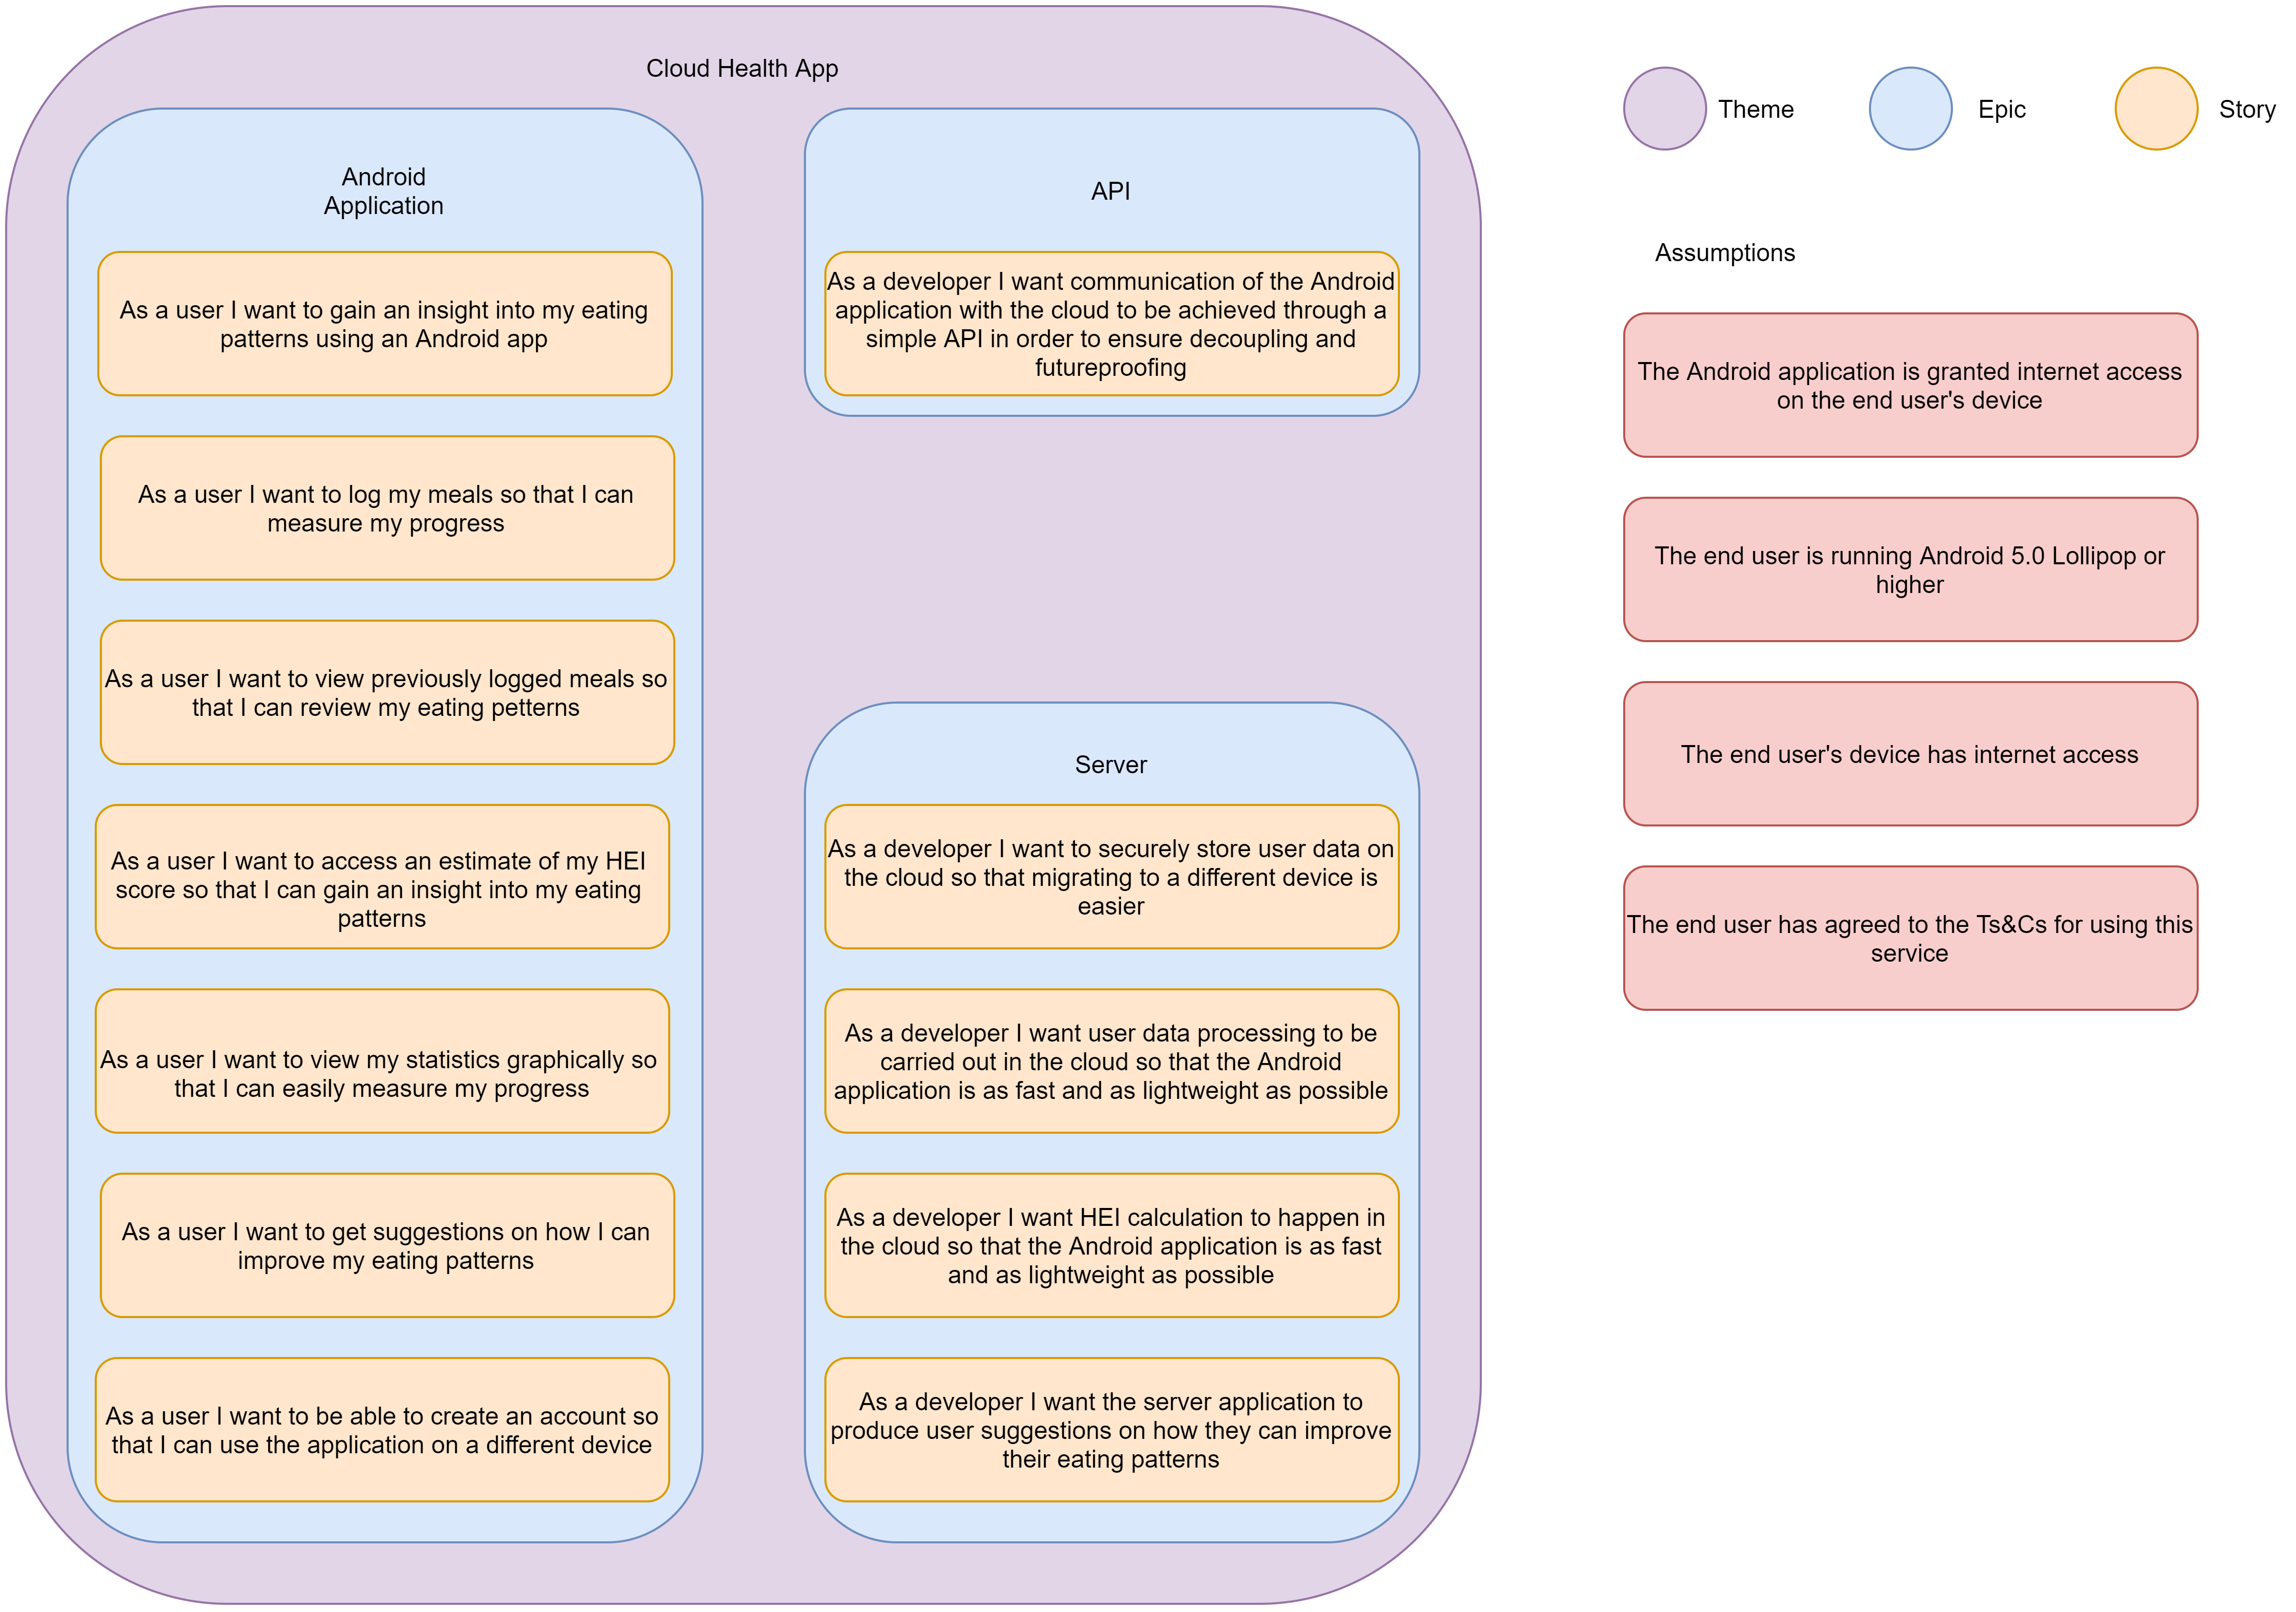
\includegraphics[width=1.3\textwidth]{backlog.png}
\centering
\caption{Product Backlog}
\label{fig:product_backlog}
\end{figure}

\bigskip
\noindent Splitting the user stories in such a way gave room for modularity and low coupling, which allowed me to work on three separate parts of the project simultaneously. Below is a brief documentation of the process of creating the application. 

\newpage
\subsection{Sprint 1}
I chose 3 stories and broke them down into tasks to begin Sprint 1, see Table \ref{table:stories_tasks_sprint_1}. 

\begin{table}[h]
\centering
\hspace*{-1.6cm}
\begin{tabular}{||m{8cm}|m{6cm}||}
\hline
    Story & Tasks \\ [0.5ex] 
    \hline
    \multirow{3}{\hsize}{As a user I want to gain an insight into my eating patterns using an Android app} & Define Fragment layouts in XML \\\cline{2-2} 
                                    & Define button layout in XML \\\cline{2-2} 
                                    & Define navigation graph  \\
    \hline
    \multirow{2}{\hsize}{As a user I want to log my meals so that I can measure my progress} & Define Fragment classes \\\cline{2-2} 
    & Define event handling for button clicks \\
    \hline
    \multirow{4}{\hsize}{As a user I want to view previously logged meals so that I can review my eating patterns} & Define Room Database \\\cline{2-2} 
    & Define the ViewModel \\\cline{2-2} 
    & Save current meals \\\cline{2-2} 
    & Load previously saved meals \\
    \hline
\end{tabular}
\caption{Stories and Corresponding Tasks for Sprint 1}
\label{table:stories_tasks_sprint_1}
\end{table}
\bigksip

\subsubsection{Defining Fragment Layouts and the Navigation Graph}
After some consideration, I decided to modify the initial design of the application layout. I chose to display all food items belonging to a meal in a single box that would expand vertically downwards as more food items would be added to it, see Figure \ref{fig:fragment_layouts}. Unnatural horizontal scrolling is thus eliminated.

\bigskip
\noindent The navigation around the application remained unchanged from the initial design. A navigation drawer accessible by swiping from the left seemed to be the most reasonable and intuitive approach, see Figure \ref{fig:navigation_label}.

\begin{figure}[h]
\centering
\hspace*{-3.5cm} 
\begin{subfigure}{.4\textwidth}
  \centering
  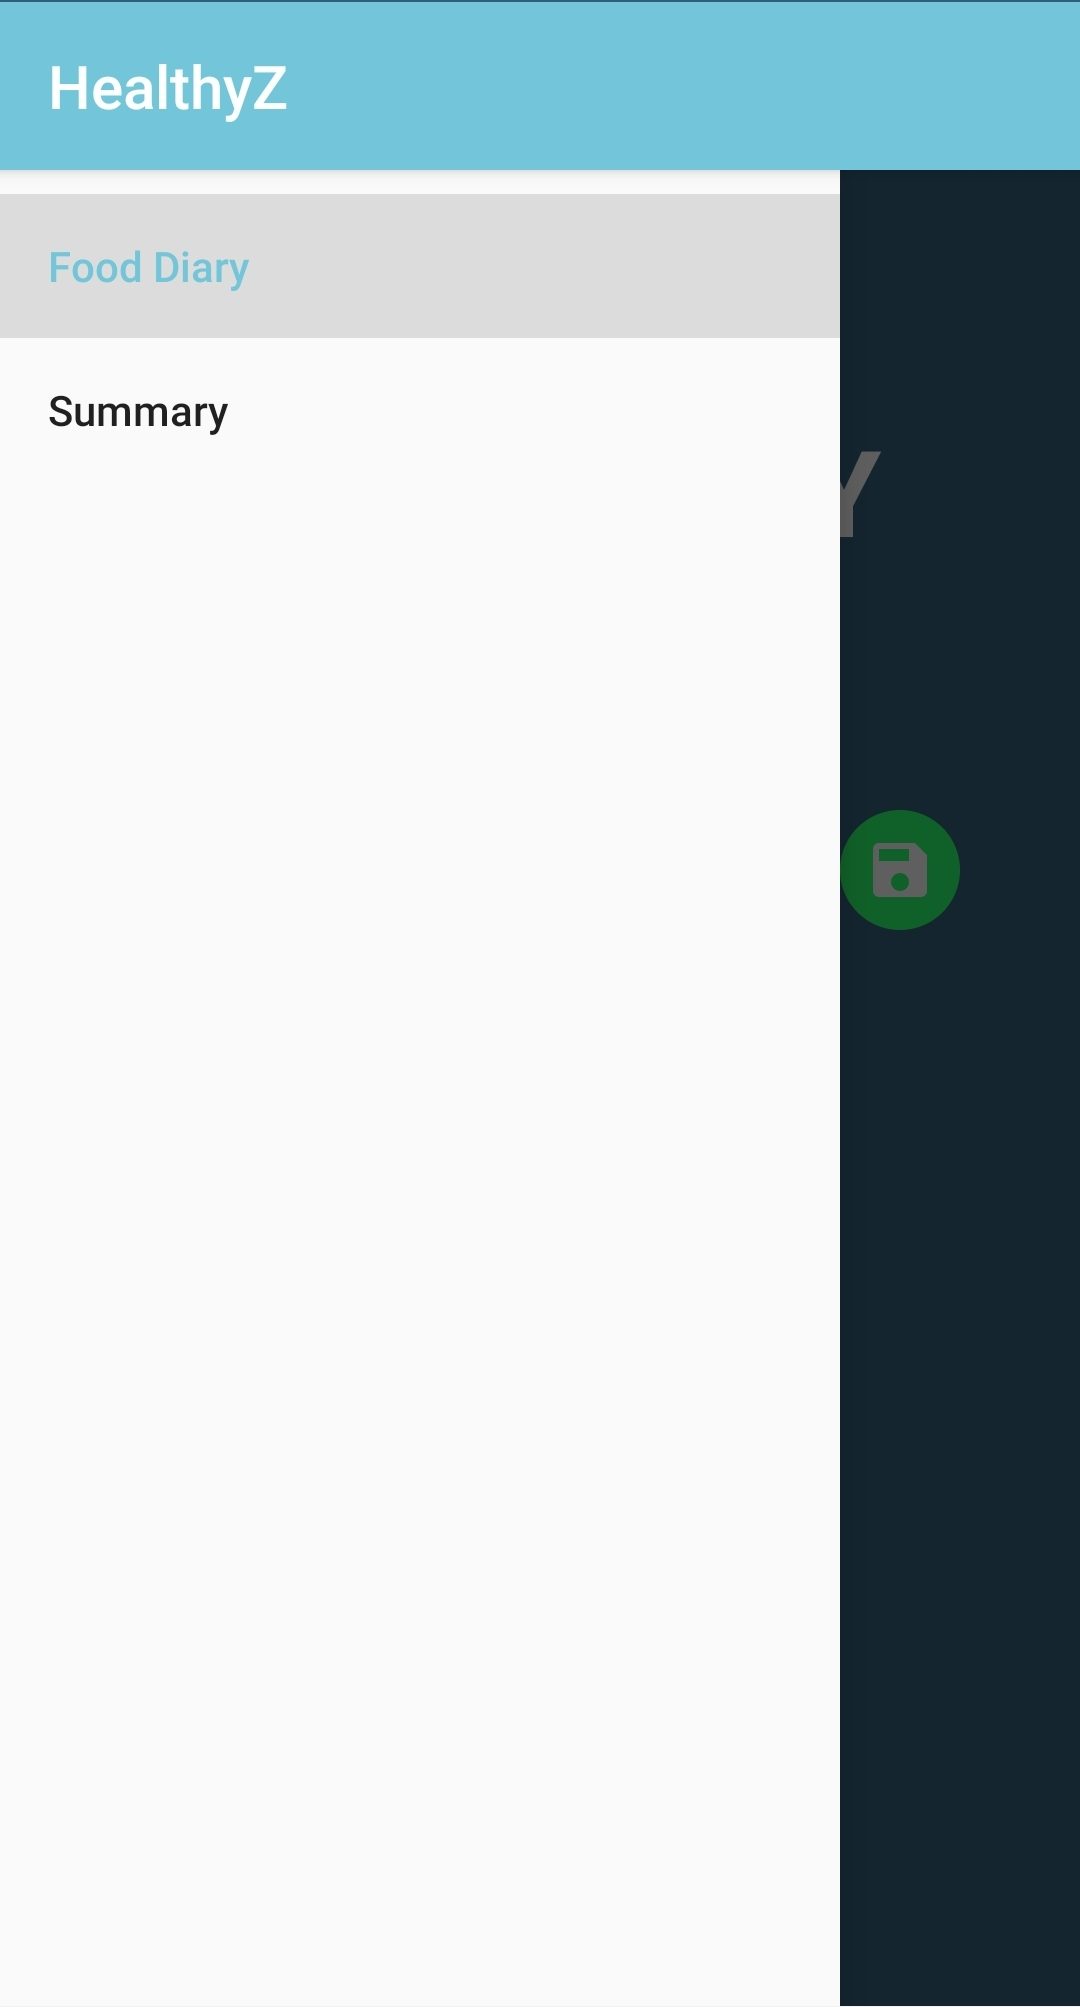
\includegraphics[height = 5.8cm]{navigation_drawer.jpg}
  \caption{Navigation Drawer}
  \label{fig:nav_drawer_label}
\end{subfigure}%
\begin{subfigure}{.4\textwidth}
  \centering
  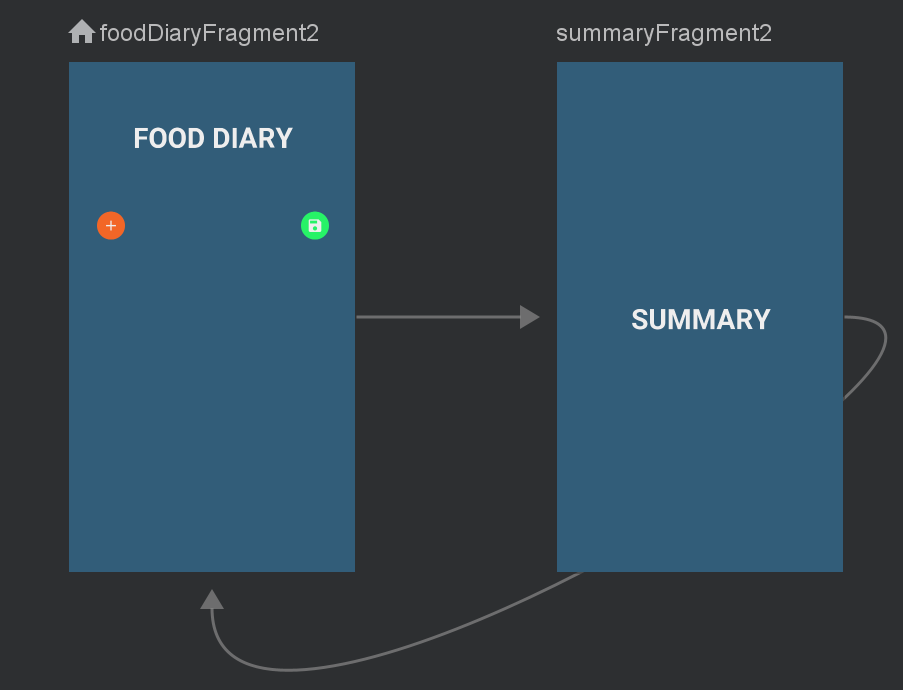
\includegraphics[height = 5.8cm]{nav_graph.png}
  \caption{Navigation Graph}
  \label{fig:nav_graph_label}
\end{subfigure}
\caption{Screenshots of the Different Screens in the Application}
\label{fig:navigation_label}
\end{figure}

\begin{figure}[h]
\centering
\hspace*{-2cm}
\begin{subfigure}{.5\textwidth}
  \centering
  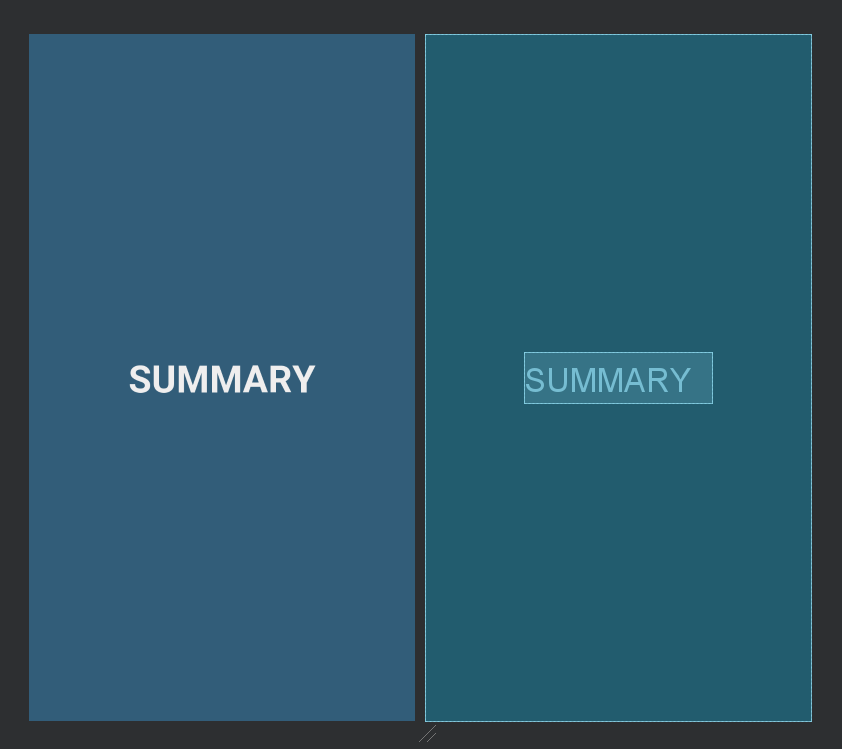
\includegraphics[width=7.5cm]{summary_fragment.png}
  \caption{Summary Fragment}
  \label{fig:summary_fragment_label}
\end{subfigure}%
\hspace*{2cm}
\begin{subfigure}{.5\textwidth}
  \centering
  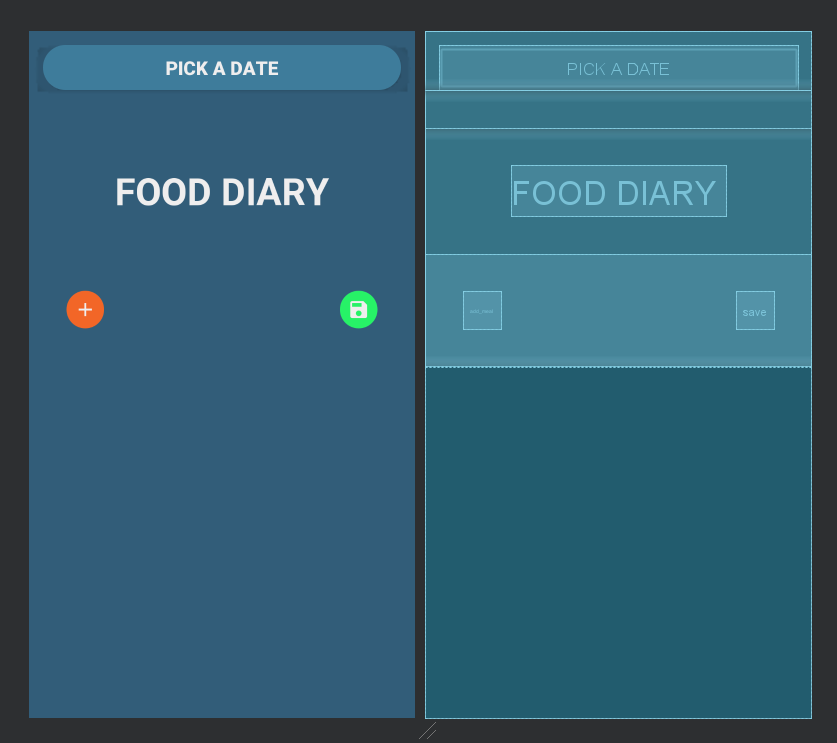
\includegraphics[width=7.5cm]{food_diary_fragment.png}
  \caption{Food Diary Fragment}
  \label{fig:food_diary_fragment_label}
\end{subfigure}
\hspace*{-4cm}
\begin{subfigure}{\textwidth}
  \centering
  
\includegraphics[width=16cm]{meal_fragment.png}
  \caption{Meal Fragment}
  \label{fig:meal_fragment_label}
\end{subfigure}
\hspace*{-4cm} 
\begin{subfigure}{\textwidth}
  \centering
  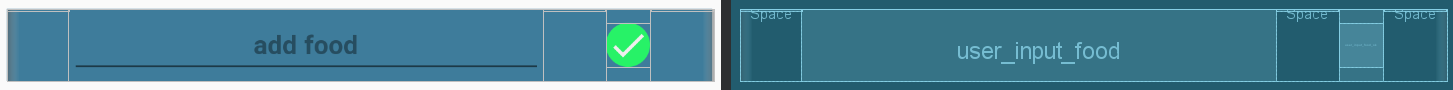
\includegraphics[width=16cm]{food_fragment.png}
  \caption{Food Fragment}
  \label{fig:food_fragment_label}
\end{subfigure}
\caption{Fragment Layouts}
\label{fig:fragment_layouts}
\end{figure}

\subsubsection{Defining Fragment Classes}
The fragment classes themselves follow the design exactly. The navigation drawer allows the user to select one of two destinations: Food Diary, or Summary page. 

\begin{itemize}
    \item \textbf{FoodDiaryFragment}: has buttons for creating a new meal (labelled with a plus symbol) and for saving the current meals to persistent storage (labelled with a tick). The FoodDiaryFragment also serves as a container for MealFragments that appear upon user request. 
    \item \textbf{MealFragment}: has a button for adding a new food item (labelled with a plus symbol). The MealFragment, similarly to FoodDiaryFragment, serves as a container for FoodFragments. 
    \item \textbf{FoodFragment}: contains a text field where the user can input a specific food item.
\end{itemize}

\newpage
\subsubsection{Event Handling}
There are 4 button layouts defined in the application, which are: 

\bigskip
\begin{itemize}
    \item \textbf{Orange Plus}: this button creates child fragment instances. A button with this layout positioned in the FoodDiaryFragment will create a MealFragment instance, and similarly a button with this layout in a MealFragment will create a FoodFragment instance, see Figure \ref{fig:orange_plus_button_layout}.
    \item \textbf{Green Save}: this button saves the user inputted meals to permanent storage, see Figure \ref{fig:green_save_button_layout}.
    \item \textbf{Green Tick}: this button saves the food item that the user inputted into the FoodFragment ,where it is located, to the ViewModel, see Figure \ref{fig:green_tick_button_layout}.
    \item \textbf{Pink Cross}: this button deletes the fragment it is in. This button can be accessed in both MealFragment and FoodFragment instances by long clicking the corresponding Orange Plus button, see Figure \ref{fig:pink_cross_button_layout}.
\end{itemize}

\bigskip
\begin{figure}[h]
\centering
\begin{subfigure}{.5\textwidth}
  \centering
  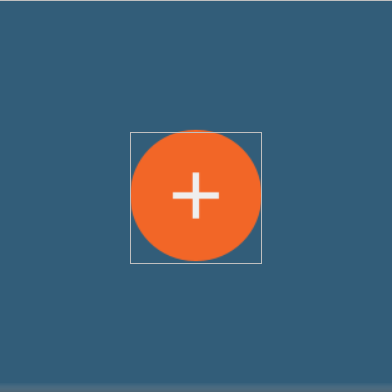
\includegraphics[width=3.5cm]{orange_plus.png}
  \caption{Orange Plus button}
  \label{fig:orange_plus_button_layout}
\end{subfigure}%
\begin{subfigure}{.5\textwidth}
  \centering
  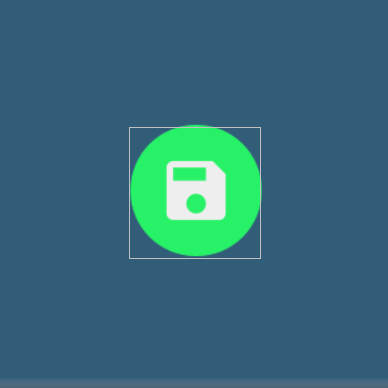
\includegraphics[width=3.5cm]{green_save.png}
  \caption{Green Save button}
  \label{fig:green_save_button_layout}
\end{subfigure}
\begin{subfigure}{.5\textwidth}
  \centering
  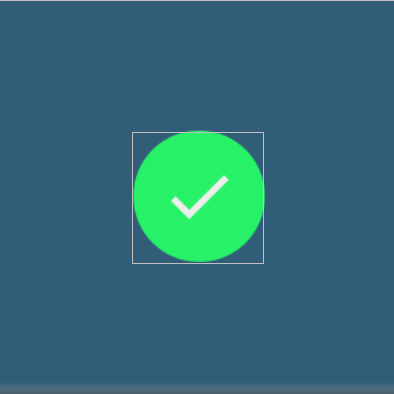
\includegraphics[width=3.5cm]{green_tick.png}
  \caption{Green Tick button}
  \label{fig:green_tick_button_layout}
\end{subfigure}%
\begin{subfigure}{.5\textwidth}
  \centering
  
\includegraphics[width=3.5cm]{pink_cross.png}
  \caption{Pink Cross button}
  \label{fig:pink_cross_button_layout}
\end{subfigure}%
\caption{Button Layouts}
\label{fig:button_layouts}
\end{figure}

\newpage
\subsubsection{Defining a Room Database}
\label{text:room_database}
Figure \ref{fig:application_overview} shows a high level overview of the application database.

\bigskip
\begin{figure}[h]
    \hspace*{-3cm} 
    
\includegraphics[height = 4cm]{ViewModel_wide.png}
    \caption{Application Overview}
    \label{fig:application_overview}
\end{figure}

\bigskip
\noindent In Figure \ref{fig:application_overview}, there are 6 distinct levels, which are: 

\bigskip
\begin{itemize}
    \item \textbf{Activity/Fragment}: this includes all the previously mentioned fragments.
    \item \textbf{MyViewModel}: the purpose of the ViewModel is to store the UI data. The ViewModel survives configuration changes, such as device rotation, during which the Activities and Fragments are destroyed and recreated, which makes it perfect for temporarily storing the user inputted meals and food items before committing to persistent storage.
    \item \textbf{MealRepository}: the repository acts as a mediator between the data source and the ViewModel. The benefit of using a repository is flexibility in future development. Adding another data source would thus only require changes to the repository, the ViewModel is unaffected. I plan to add cloud storage as a second data source later on.
    \item \textbf{MealDao interface}: annotated with '@Dao', this interface is used to interact with the database. Methods defined in the interface are attached to SQLite queries that are executed when their corresponding methods are called.
    \item \textbf{Meal entity}: annotated with '@Entity', this class represents a row in the database, with getters and setters for the columns in that row. 
    \item \textbf{MealRoomDatabase}: annotated with '@Database', this implementation of a Room database follows a singleton design pattern in order to ensure that it is accessed correctly. Singleton design pattern is allowing only one instance of a class to be made. This is sufficient for such a small application as the database will not be accessed from multiple different parts of the application simultaneously. 
\end{itemize}

\subsubsection{Defining a ViewModel}
MealFragments are assigned IDs when they are first created so that they can be saved and recreated later. The ID counter is kept in the MyViewModel class, ensuring unique IDs for MealFragments. FoodFragments receive the ID from their parent MealFragment upon creation. MyViewModel class contains a map of integers to lists of strings. User inputted food item is added as a string to the list mapped to by the value of the meal ID in the map stored in the MyViewModel class.

\bigskip
\subsubsection{Saving and Loading User Data}
I implemented a simple date picker so that the user could change previously entered meals. I implemented the DatePickerDialog interface in the FoodDiaryFragment class in a way that causes the date picker to pop up when the user presses the 'Pick a Date' button at the top of the FoodDiaryFragment. I chose a colour scheme that was consistent with the rest of the application. See Figure \ref{fig:date_picker} for a screenshot of the date picker dialogue.

\begin{figure}[h]
    \centering
    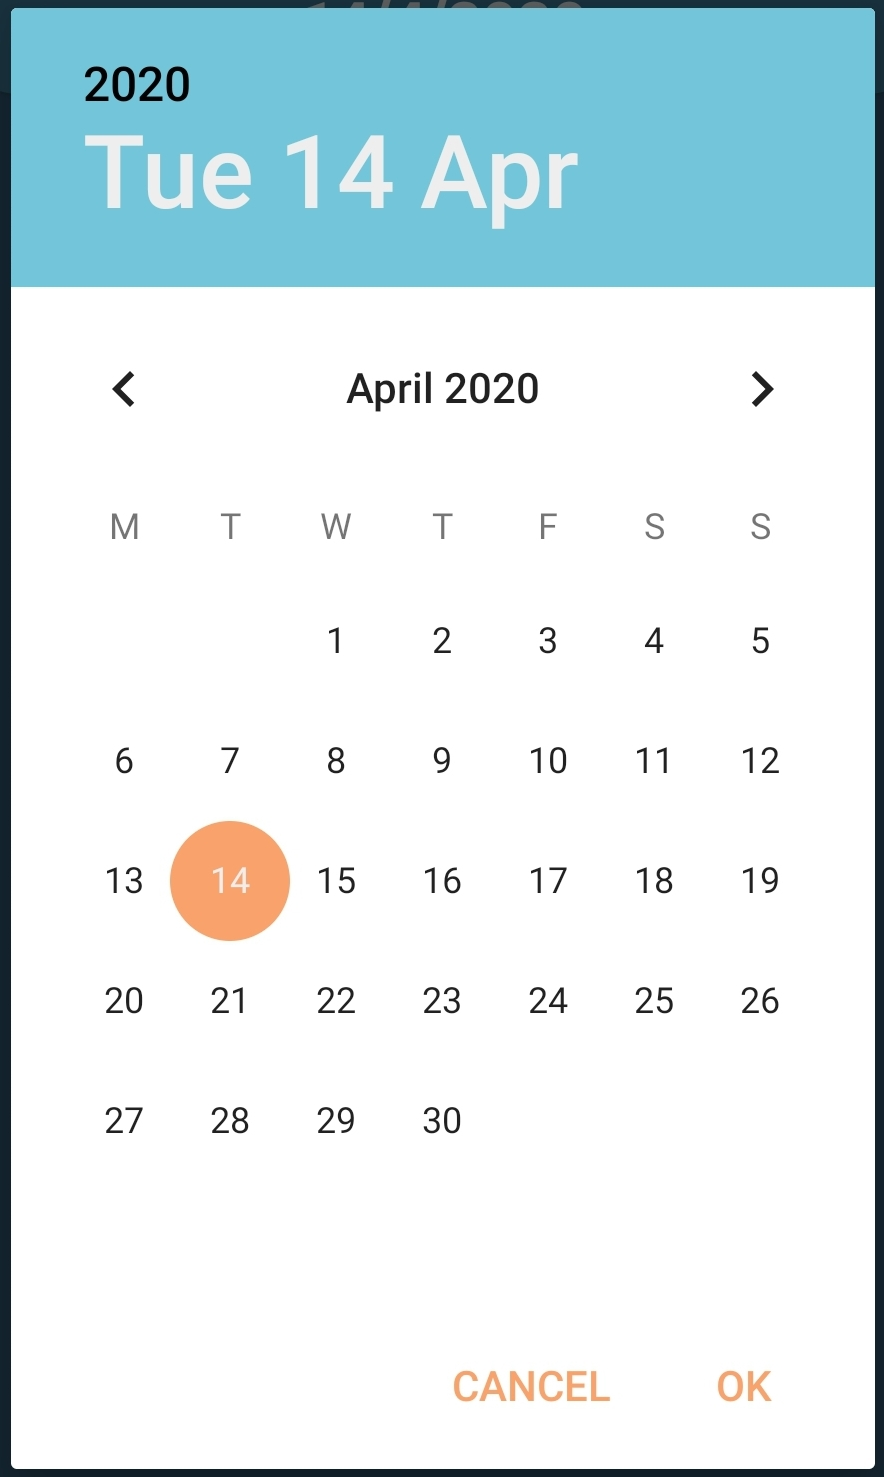
\includegraphics[width = 4.5cm]{date_picker.jpg}
    \caption{Date Picker}
    \label{fig:date_picker}
\end{figure}

\bigskip
\noindent MyViewModel class has a date variable, the default value of which is the current date. The date variable is used to retrieve data from the SQLite database. When a user picks a different date in the date picker, the date variable in MyViewModel is updated and meals from the new date are loaded. Clicking the green save button (see Figure \ref{fig:green_save_button_layout}) causes data stored in MyViewModel class to be saved to the SQLite database.

\subsection{Sprint 2}
At this point, I needed to develop the back-end of the application. The second sprint consisted of stories from the 'Server' epic in the product backlog, see Table \ref{table:stories_tasks_sprint_2}.

\begin{table}[h]
\centering
\hspace*{-2.1cm}
\begin{tabular}{||m{6cm}|m{9cm}||}
\hline
    Story & Tasks \\ [0.5ex] 
    \hline
    \multirow{3}{\hsize}{As a developer I want to securely store user data on the cloud so that migrating to a different device is easier} 
                                    & Create SQLite database for storing user data \\\cline{2-2} 
                                    & Create SQLite table for storing user input \\\cline{2-2} 
                                    & Create SQLite table for storing user food set \\\cline{2-2}
                                    & Create SQLite table for storing user food set by date\\
    \hline
    As a developer I want user data processing to be carried out in the cloud so that the Android application is as fast and as lightweight as possible & Generate food set from user input for every user in the dataset \\
    \hline
    \bigskip
    \multirow{3}{\hsize}{As a developer I want HEI calculation to happen in the cloud so that the Android application is as fast and as lightweight as possible} & Create a fuzzy string matching program \\\cline{2-2} 
    & Use fuzzy string matching program to match user inputted food items in food set to a food item in the FNDDS database \\\cline{2-2} 
    & Calculate an estimate of the scores of the HEI components by using the matched foods from the FNDDS, using nutritional data from FNDDS and FPED databases \\
    \hline
\end{tabular}
\caption{Stories and Corresponding Tasks for Sprint 2}
\label{table:stories_tasks_sprint_2}
\end{table}
\bigksip

\subsubsection{Creating an SQLite Database for Storing User Data}
Figure \ref{fig:user_database_model} shows the tables in the MyFitnessPal database that was created, as well as the FNDDS and FPED databases that were required for this project:

\begin{itemize}
    \item \textbf{FoodDiary}: this table contains a list of foods and its nutritional value stored in a JSON format. The primary key is the entry ID. The reason for this is the fact that neither one of user ID, date, food list, daily goal, nor any combination of those fields could serve as a key as they're not unique.
    \item \textbf{DateFoodSetNut}: this table contains every user's set of foods and their nutritional values for every recorded day.
    \item \textbf{FoodSetNut}: this table contains every user's set of foods and their nutritional values for the entirety of the time the user kept the food diary. 
    \item \textbf{FNDDS}: this table is the official FNDDS database as supplied by USDA.
    \item \textbf{FPED}: this table is the official FPED database as supplied by USDA.
\end{itemize}

\noindent Both FPED and FNDDS tables were contained in Microsoft Access Database files with the same names. These databases contain detailed nutritional information of nearly 9000 food items.

\begin{figure}[h]
    \centering
    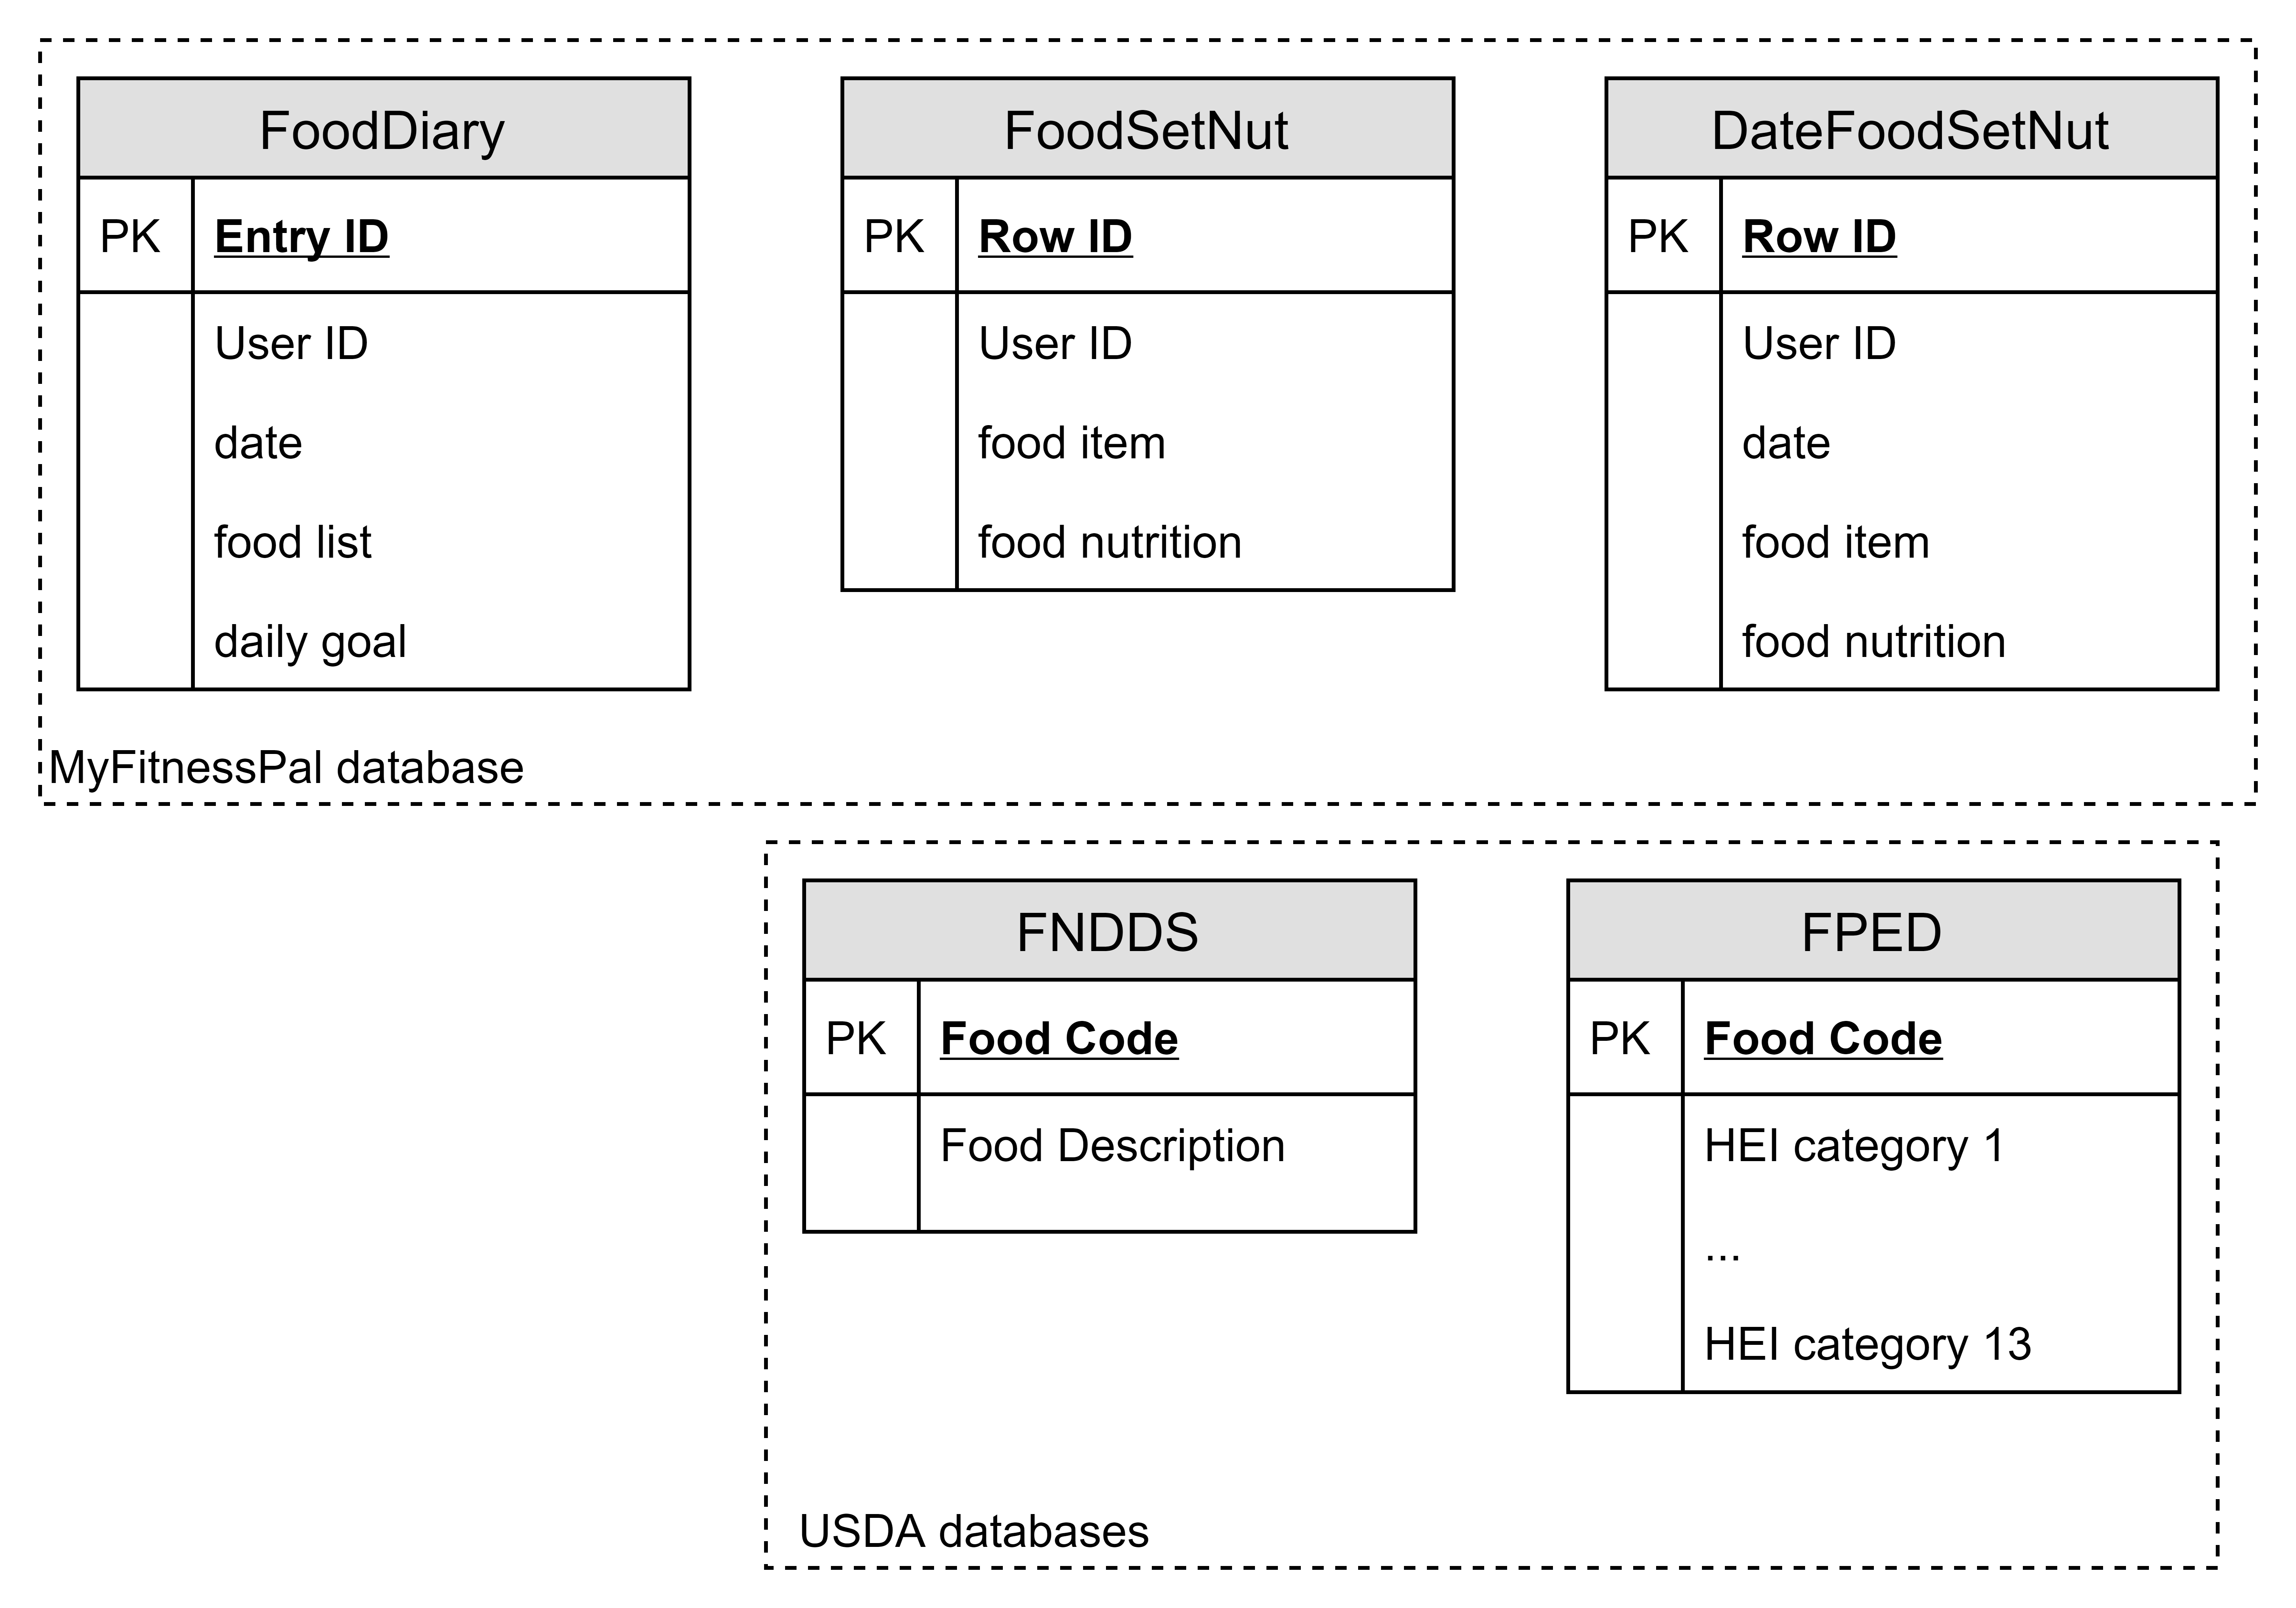
\includegraphics[width = 10cm]{user_database_model.png}
    \caption{User Database Model}
    \label{fig:user_database_model}
\end{figure}


\subsubsection{Generating Food Sets for Every User}
The first table I populated was the FoodDiary table. I created a parser for the MyFitnessPal data set \cite{diet_success_predictions} and put every single line from the tab-separated file into a row in the FoodDiary table. 

\bigskip
\noindent I then populated the FoodSetNut table by retrieving every single food item of the user input from the FoodDiary table, which added it to a map of the food item name (as a string) to that food item's nutritional value (as a string). Using a map to store the user data eliminated any duplicates, resulting in the food set of interest, which was then saved to the FoodSetNut table. Similarly, the DateFoodSetNut table was populated, but for every recorded day.

\subsection{Fuzzy String Matching}
The food items in MyFitnessPal data set \cite{diet_success_predictions} were formatted consistently, thus making it possible to efficiently clean the input. This was achieved by deleting unnecessary information about portion size, removing any brackets, numbers and non-alphabetical characters, and changing the input to lower case. Lastly, Porter Stemmer implementation from Apache OpenNLP library \cite{apache_opennlp} was used to stem every word in the description. 

\bigskip
\noindent My initial attempt was to use Levenshtein distance (see section 5.2.6 'String Comparison Metrics') as a metric to match user input to the closest food item in the FNDDS database. The problem with this approach was word order. Changing the word order would result in a low similarity score, which is undesirable.

\bigskip
\noindent Instead, a slightly modified version of the Mongue-Elkan algorithm was implemented (see section 5.2.7 'String Matching'). In my implementation of this algorithm, the string similarity was computed in the following way: 

\begin{itemize}
    \item For every word in the shorter sentence, assign a word from the longer sentence with the lowest Levenshtein distance. 
    \item Return the sum of these distances. 
\end{itemize}

\bigskip
\noindent The difference here was that my implementation was a one-to-one mapping. A word in the longer sentence could map to at most one word in the shorter sentence. Additionally, my implementation is symmetric, whereas the original algorithm is not \cite{mongue_elkan}. 

\subsubsection{Matching User Input to a Food Item in the FNDDS}
In order to calculate the HEI score, I chose to take advantage of the available databases. FNDDS contains nearly 9000 food items with an in-depth description and nutritional information. I simplified the process of estimating the HEI score by finding the closest match of the user input to a food item in the FNDDS database using the fuzzy string matching program to calculate string similarity, and returning the most similar FNDDS food item. The food code associated with the match in the FNDDS was used to find the required information to calculate the HEI score in the FNDDS and FPED databases. 

\subsubsection{Estimating HEI Score}
\noindent According to the 2015 HEI Update \cite{hei_2015}, the three basic steps in calculating the HEI score are : 

\begin{enumerate}
    \item Identifying a set of foods
    \item Determining amounts of dietary constituents
    \item Deriving ratios and scoring against the 2015 HEI standard
\end{enumerate}

\noindent For every user input, I identified the closest food item in the FNDDS database using the fuzzy string matching program. From the FNDDS, the food code, amount of saturated fats, energy content, sodium content, monounsaturated fats and polyunsaturated fats were extracted for every match. The food code was then used to retrieve all the values of the necessary components in calculating the HEI score from the FPED database. In order to determine the amounts of the dietary constituents, I multiplied the values from the FPED by the ratio of calories the user input to the calories obtained from the FNDDS for a particular food item. In this way, the portion sizes were estimated.

\bigskip
\noindent Summing the relevant values up and comparing to the 2015 HEI standards resulted in an estimate of that user's HEI score, based on all the food that they entered. 

\subsection{Sprint 3}
At this point, I needed to implement a visual representation of the HEI score. This is commonly achieved with a radar graph. The stories and their corresponding tasks are displayed in Table 6.

\begin{table}[h]
\centering
\hspace*{-2.1cm}
\begin{tabular}{||m{6cm}|m{9cm}||}
\hline
    Story & Tasks \\ [0.5ex] 
    \hline
    As a user I want to access an estimate of my HEI score so that I can gain an insight into my eating patterns & Display HEI score numerically in the application\\
    \hline
    As a user I want to view my statistics graphically so that I can easily measure my progress & Implement a radar graph for the HEI score in the application \\
\hline
\end{tabular}
\caption{Stories and Corresponding Tasks for Sprint 3}
\label{table:stories_tasks_sprint_3}
\end{table}

\subsubsection{Implementing a Radar Graph}
A great visual way of displaying the HEI score is in a radar graph with 13 branches, where every branch corresponds to one of the 13 HEI components.

\bigskip
\noindent MPAndroidChart library \cite{library_mpandroidchart} allowed me to efficiently implement an aesthetically pleasing radar graph. Using the libraries documentation, I added a radar graph following the general colour theme of the application to the summary page. 

\bigskip
\noindent At this point, the server-side has not yet been implemented. For testing purposes, a random HEI score, stored as an array of doubles, was hard-coded in MyViewModel. The HEI score could be retrieved from the cloud by the MealRepository instance associated with MyViewModel once the server-side was implemented. A getter method returning the HEI score array was implemented in MyViewModel, which is called when the user navigates to the summary page of the application, where the radar graph displays the HEI score. See Figure \ref{fig:numerical_hei_scores} for screenshots of the application with the numerical scores visible and hidden. 

\subsubsection{Displaying HEI Score Numerically}
Due to the size constraints of the application running on a smartphone, I chose to present the individual scores of the HEI components in a table. Furthermore, as the HEI scores are only estimations and thus not precise, I would like to draw the user's attention to the radar graph displaying the overall trend and away from the numerical values. The HEI score table is hidden by default, its visibility is toggled by pressing the corresponding orange button. 

\begin{figure}[h]
\centering
\hspace*{0.75cm} 
\begin{subfigure}{.4\textwidth}
  \centering
  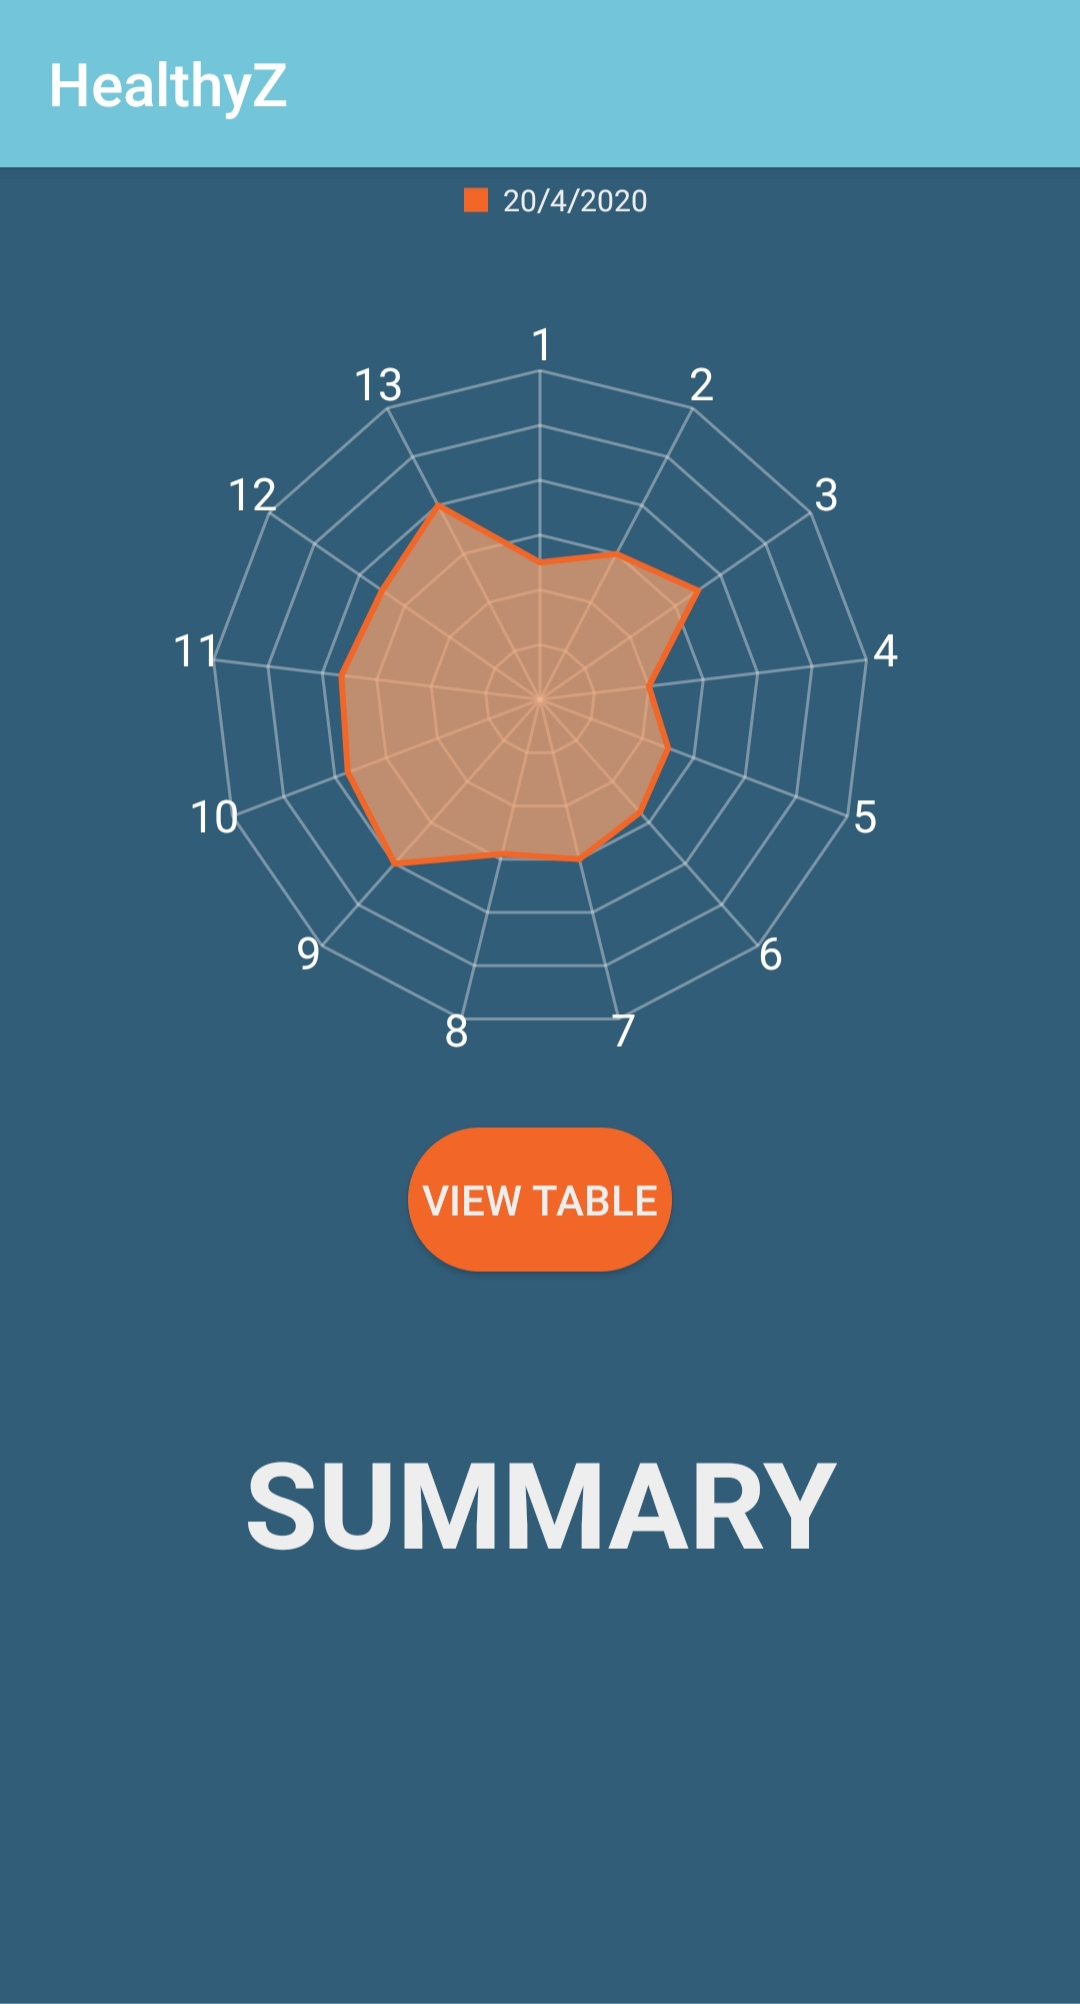
\includegraphics[width = 4.05cm]{hei_table_invisible.jpg}
  \caption{HEI Score Table is Hidden}
  \label{fig:hei_table_invisible}
\end{subfigure}%
\begin{subfigure}{.4\textwidth}
  \centering
  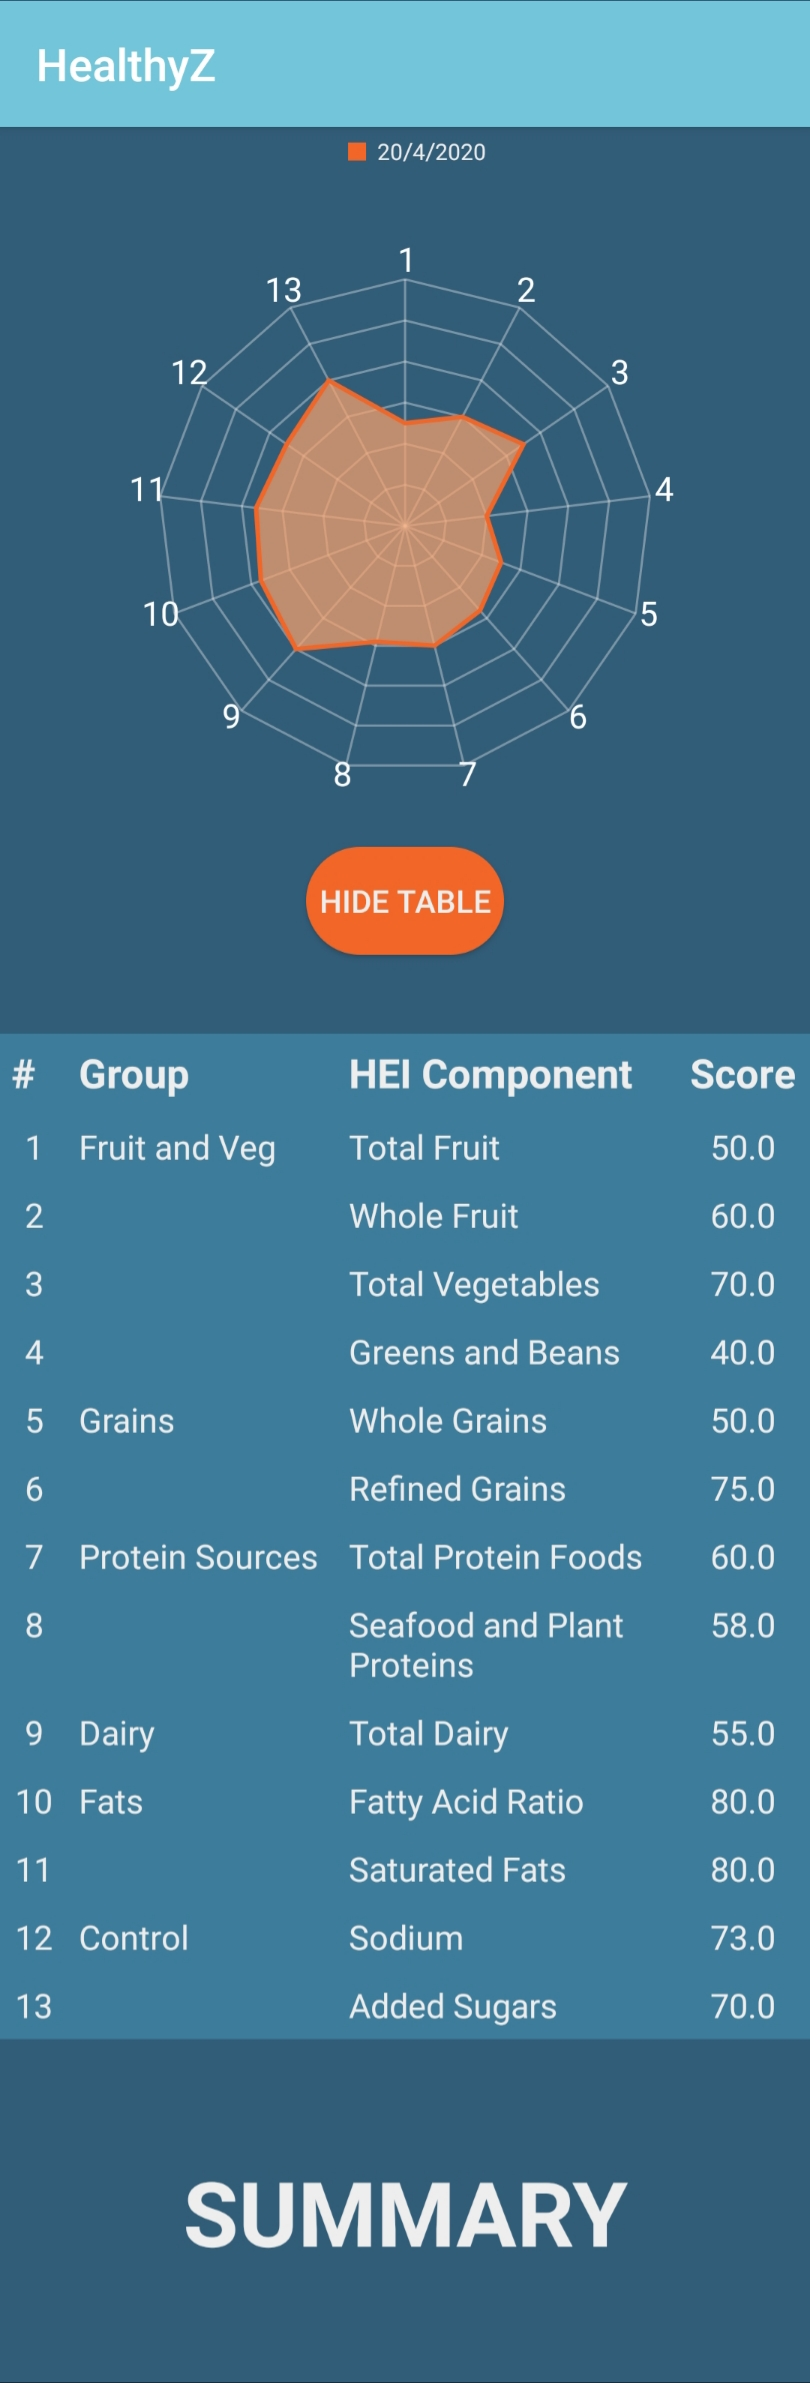
\includegraphics[height = 7.515cm]{hei_table_visible.jpg}
  \caption{HEI Score Table}
  \label{fig:hei_table_visible}
\end{subfigure}
\caption{Screenshots of the Summary Page in the Application \newline (Each Branch in the Radar Graph Corresponds to a HEI Component)}
\label{fig:numerical_hei_scores}
\end{figure}

\subsection{Sprint 4}
At this point, there was a slight miss alignment in the project. The back-end code calculating an estimate of a user's HEI utilised the additional nutritional information of the recorded food items in the MyFitnessPal dataset \cite{diet_success_predictions}. The number of calories was necessary to estimate the portion size, and the salt content was to be used later for evaluation. This caused a reevaluation of the product backlog and redesign of feature implementations, see Table \ref{table:stories_tasks_sprint_4}.

\begin{table}[h]
\centering
\hspace*{-2.1cm}
\begin{tabular}{||m{6cm}|m{9cm}||}
\hline
    Story & Tasks \\ [0.5ex] 
    \hline
    \multirow{2}{\hsize}{As a developer I want to gather additional nutritional information in order to calculate the HEI estimate} 
                                            & Add calorie and sodium input boxes in the FoodFragment \\\cline{2-2}
                                            & Update MyViewModel and MealRepository classes to store the user input as JSON objects \\
    \hline
    \multirow{4}{\hsize}{As a developer I want the user to store the HEI score locally, minimising server usage and optimising loading speeds}
                                                        & Update project structure \\\cline{2-2}
                                                        & Create a new Entity class for the HEI score \\\cline{2-2}
                                                        & Create a DAO class for accessing the HEI score \\\cline{2-2}
                                                        & Update the MealRoomDatabase class to contain two tables, for storing user input and HEI score \\
\hline
\end{tabular}
\caption{Stories and Corresponding Tasks for Sprint 4}
\label{table:stories_tasks_sprint_4}
\end{table}

\subsubsection{Updating Project Structure}
I decided to give the android application project some structure. As I was developing the application using the MVVM architecture, I decided to split the classes into packages based on the purpose they were serving.

\begin{figure}[h]
\centering
\includegraphics[width=8cm]{MVVM Structure.png}
\caption{Application Structure}
\label{fig:application_structure}
\end{figure}

\bigskip
\noindent Figure \ref{fig:application_structure} shows the updated design of the application architecture, with all the classes being split into sub-packages based on their purpose. All the classes responsible for the UI were placed in the 'view' package and similarly, the classes responsible for handling data were placed in the 'viewmodel' package. I split the classes responsible for data storage and retrieval into two packages, the 'database' package contained classes for local data storage, and the 'server' package contained classes for connecting to the server. 

\bigskip
\noindent Splitting the classes into sub-packages provided an additional layer of abstraction. The MealRoomDatabase class follows the singleton design pattern to ensure correct usage. The instance of the database is package protected, and thus directly inaccessible from the other packages. It can only be accessed with the public methods declared in the MealRepository class, thus providing extra security on its correct usage. 

\subsubsection{Altering the Application Layout}
I redesigned the application layout to allow the user to input calorie and sodium intake, as this information is required for HEI calculations, and later for evaluation. Alternatively, it would be possible to allow the user to input very detailed nutritional information, such as including protein, fat and carbohydrate intake also. This would make the application UI too messy, however. The minimum information required to perform the calculations is collected.

\bigskip
\noindent I added two input boxes in the FoodFragment. I then changed the green tick button event handling slightly, to ensure that the user inputted a number in both the calorie and sodium input boxes, see Figure  \ref{fig:updated_food_fragment}.

\begin{figure}[h]
    \centering
    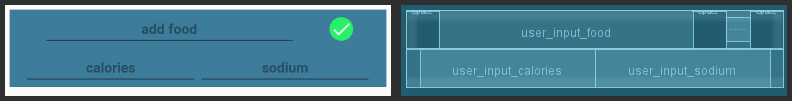
\includegraphics[width = 12cm]{food_fragment_updated.png}
    \caption{Updated FoodFragment}
    \label{fig:updated_food_fragment}
\end{figure}

\subsubsection{Updating ViewModel}
Previously, user input was stored in MyViewModel class in a map of integers to lists of strings, where the integer was the meal ID and the list of strings was the list of user inputted food items. With the addition of calorie and sodium intake information, this could no longer work. I chose to store the user input in JSON format, with the attributes 'food\_item', 'calories' and 'sodium' being assigned the values that the user inputs. I proceeded to update MyViewModel class to map integers to lists of JSON objects. An alternative to lists would be to simply map integers to JSON arrays. I made a compromise by keeping lists, which reduced the amount of code I had to rewrite. 

\bigskip
\noindent JSON format was optimal, as it is serializable. This meant that I could leave the Meal entity class and MealDao interface unchanged, whilst retaining the useful functionality of the JSON Java objects in the rest of the project. Additionally, JSON is often used to transfer data, thus storing the user input in a JSON format would reduce the amount of work required to upload the user's food diary to the server for HEI calculations. 

\subsubsection{Storing HEI Scores locally}
In order to minimise server usage and optimise loading speeds of the application, I chose to store the calculated HEI scores locally. This was achieved in the same way as with the user input information, described in section 8.2.4 'Defining a Room Database'. I took the following steps: 

\begin{itemize}
    \item \textbf{Create HEIRecord class}: annotated with '@Entity', this class is used to set and retrieve field values in the corresponding table contained in the MealRoomDatabase.
    \item \textbf{Create HEIRecordDao interface}:  annotated with '@Dao', this interface defines the API for interacting with the table.
    \item \textbf{Update MealRoomDatabase class}: I added the HEIRecord to the entity declaration so that RoomDatabase superclass creates two tables for storing user input and HEI scores. 
    \item \textbf{Update MealRepository class}: I implemented the methods defined in the HEIRecordDao interface and made them publicly accessible.
\end{itemize}

\subsection{Sprint 5}
Having coded the foundations of the back-end and front-end, it was then time to begin bringing it together by establishing communication between the android application and the server. Stories and their corresponding tasks are displayed in Table \ref{table:stories_tasks_sprint_5} 

\begin{table}[h]
\centering
\hspace*{-2.1cm}
\begin{tabular}{||m{6cm}|m{9cm}||}
\hline
    Story & Tasks \\ [0.5ex] 
    \hline
    \multirow{5}{\hsize}{As a developer I want communication of the Android application with the cloud to be achieved through a simple API in order to ensure decoupling and future-proofing} 
                                & Set up a Docker container with TomCat and SQLite \\\cline{2-2}
                                & Implement a Java Servlet for running the HEI calculations and returning the estimated HEI score as a JSON object \\\cline{2-2}
                                & Implement a Java Servlet for allocating a user ID to an individual user \\\cline{2-2}
                                & Implement a Java Servlet for saving the user input on the server \\\cline{2-2}
                                & Implement an API for accessing and executing relevant calculations, independent of the code for these calculations \\
\hline
\end{tabular}
\caption{Stories and Corresponding Tasks for Sprint 5}
\label{table:stories_tasks_sprint_5}
\end{table}

\subsubsection{Setting Up a Docker Container}
Having researched multiple different server software, I decided that Apache Tomcat \cite{apache_tomcat} would be the most suitable for this project, as it provides a Java environment for web applications. In order to ensure future-proofing and to simplify the development process, I decided to deploy the application inside a Docker container \cite{docker}, as this would allow the application to be deployed with ease from any machine. IntelliJ ULTIMATE integrated development environment \cite{intellij} contains built-in support for using Docker containers. The latest TomCat docker container was pulled with 'docker pull tomcat' command. SQLite was then installed in the container, which made it ready for deployment.

\subsubsection{Implementing a Servlet for Allocating a User ID}
The purpose of a servlet is to handle HTTP requests. My servlet classes extended the HttpServlet from Java Platform Standard Edition 7. 

\bigskip
\noindent Allocating the user ID based on the next available ID from the database would ensure unique identification of users. Due to the large size of the tables in the database, finding the maximum value of the user ID column in any table was a time-consuming process. To speed up the process, I inserted an entry at the start of the FoodDiary table with values 'entry\_id'=-1, 'user\_id'=MAX(user\_id) and NULL for the other columns. This entry would never be used in any calculations, and it contains the highest 'user\_id' in the records. When a new user is created, the 'user\_id' value in this entry is retrieved, incremented, and assigned to the new user. This entry is then updated with the new, incremented value of the highest 'user\_id' in the records. A more practical approach would be to use a user-chosen login, nickname, or email address, however, as I do not have such information for all the users in the MyFitnessPal dataset \cite{diet_success_predictions}, I chose to use numbers. 

\subsubsection{Implementing a Servlet for Uploading User Input}
Changing the Android application to save the user input in JSON format had the additional benefit of simplifying the process of uploading the user's food diary to the server; JSON is serializable and thus a popular choice of data format for data transfer. 

\bigskip
\noindent I proceeded to implement a servlet that receives a JSON array containing user input information. This JSON array was then automatically saved to the 'DateFoodSetNut' table. In order to guarantee data freshness, any existing data for the 'userID' and 'date' parameters specified in the HTTP request is deleted from 'DateFoodSetNut' prior to insertion of the fresh data. 

\subsubsection{Implementing a Servlet for HEI Calculations}
I implemented a Java servlet that calculated the HEI score, based on the parameters specified in the HTTP request. Supplying 'userID' and
'date' parameters in the query would run the previously implemented Java code (see section 7.5.2 Estimating HEI Score) and return a JSON array of the 13 HEI components and the actual sodium intake of the user from the MyFitnessPal dataset \cite{diet_success_predictions}. For this calculation, the food items and their nutritional values are retrieved from 'DateFoodSetNut' table.

\subsubsection{Implementing a Server API}
Tomcat servers have a 'web.xml' configuration file, which maps URIs to servlets \cite{apache_tomcat_web_xml}. Giving the aforementioned servlets clear and descriptive mappings makes it easy to execute them. For example, 'UploadServlet' has a servlet mapping of '/upload'.

\subsection{Sprint 6}
At this point, I had enough data and resources to begin implementing the recommender system. See Table \ref{table:stories_tasks_sprint_6}

\begin{table}[h]
\centering
\hspace*{-2.1cm}
\begin{tabular}{||m{6cm}|m{9cm}||}
\hline
    Story & Tasks \\ [0.5ex] 
    \hline
    \multirow{4}{\hsize}{As a developer I want the server application to produce user suggestions on how they can improve their eating patterns} 
                                & Implement K-Means clustering algorithm \\\cline{2-2}
                                & Generate feature vectors for every user in the MFP dataset \\\cline{2-2}
                                & Implement collaborative filtering by generating a list of foods that other users in the cluster have eaten in the past \\\cline{2-2}
                                & Filter the list of foods to produce food items maximising the user's HEI score \\
    \hline
    As a user I want to get suggestions on how I can improve my eating patterns & Change the layout of the SummaryFragment in the Android application to display a list of suggested food items \\
    \hline
\end{tabular}
\caption{Stories and Corresponding Tasks for Sprint 6}
\label{table:stories_tasks_sprint_6}
\end{table}

\subsubsection{Implementing K-Means Clustering Algorithm}
The K-Means implementation takes a list of 'User' objects containing the user ID and feature vector, the number of clusters 'k', and the number of iterations the algorithm should be executed. 

\bigskip
\noindent Clustering is performed by randomly generating 'k' many centroid vectors, assigning the feature vector of every 'User' object to the closest centroid and then updating the centroid to be the mean vector of all the vectors assigned to it. If a cluster is empty, its centroid is assigned a randomised value.

\bigskip
\noindent This process is repeated for a specified number of iterations and a list of 'User' objects from the same cluster as the 'User' of interest is returned. Theoretically, this list of users would contain users with similar food preferences to the user of interest. The list of foods that they eat can then be extracted and used as a basis for the recommendations.

\subsubsection{Generating Feature Vectors for Users in Dataset}
'FoodSetNut' table in the database contains the set of foods a user consumed to date. I believe that such a set of foods is likely to be representative of the user's food preferences. I chose to disregard the frequency of consumption of a specific food item, as I do not think it is reflective of the user's liking of that food. 

\bigskip
\noindent A user may really like a dish, but consume it infrequently as it is expensive or energy-dense. On the contrary, a user may force themselves to regularly consume a food item for its health benefits, despite disliking its taste. Using a set of foods eliminates that problem, however the direct consequence of this is that foods that the user ate just once and really disliked will also, unfortunately, affect the user profile.

\bigskip
\noindent The data is likely to be biased. People who are willing to track their food consumption are likely to be more health-conscious than the average person, and as a result, may alter their diet. It is also important to note that the MyFitnessPal dataset \cite{diet_success_predictions} has been collected through the years 2014 and 2015. Social media influence has been found to affect health consciousness of young adults \cite{getting_healthy}. The changes in social media popularity since 2014-2015 could have also had an effect on the relevance of the dataset. 

\bigskip
\noindent I recognise that biological and environmental factors are going to affect a persons diet. Allergies, financial status and even geographical location may play a role in the availability and consumption of certain food items. Taking such factors into consideration is outside of the scope of this project. For the above reasons, the following assumptions have been made: 

\begin{table}[h]
\centering
\hspace*{-0.75cm}
\begin{tabular}{||m{0.5cm}|m{11.5cm}||}
\hline
    ID & Assumption \\ [0.5ex] 
    \hline
    1 & Set of foods a user consumed throughout the duration of the data collection is representative of their food preferences.\\
    \hline
    2 &  Every user had access to foods they like.\\
    \hline
    3 &  Social media influence on the health consciousness of the average person has not significantly changed since the collection of the dataset.\\
    \hline
    4 &  Geographical location of a user did not have a significant impact on their diet due to globalisation.\\
\hline
\end{tabular}
\caption{Assumptions Made in Recommender System Design}
\label{table:recommender_system_assumptions}
\end{table}

\bigskip
\noindent 'FoodSetNut' table in the database contains columns 'food\_item', which contains a description of the food item in the food set, and 'WWEIA\_code', which is the corresponding WWEIA category code of the matched food item from the FNDDS database. There are 155 unique WWEIA food categories. 

\bigskip
\noindent A feature vector for a user was generated by constructing a bit vector of size 150, where the index of a bit would correspond to one of the WWEIA food categories. The set of WWEIA codes for a user is retrieved from the database. For every WWEIA code in the set, the bit at the index corresponding to that WWEIA code was set to 1, and all other bits set to 0. If the set of WWEIA food categories for a user is A, then: 

\begin{align*}
    vector &= [x_1,x_2..x_{155}]
\end{align*}

\[
    x_{i \in \{1..155\}} = 
\begin{cases}
    1,& \text{if } WWEIA_i \in A\\
    0,& \text{otherwise}
\end{cases}
\]

\bigskip
\noindent Given the limited resources at hand, and having made the aforementioned assumptions, I believe that this feature vector suffices. The amount of possible feature vectors of this kind is 2\textsuperscript{155} , which is 4.57e+46 to three significant figures. The dataset contains 9897 users, which means it is incredibly unlikely that any two users will have the same feature vector.

\subsubsection{Vector Similarity Measure}
Euclidean distance and cosine similarity are two metrics I considered. The formulae for Euclidean distance and cosine similarity of two vectors are:

\begin{align*}
    Euclidean(\vec{u},\vec{v}) = \sqrt{\sum_{i=1}^{n} ({\vec{u_{i}}-\vec{v_{i}}})^2} = \sqrt{|\vec{u}|^{2} + |\vec{v}|^{2} - 2\vec{u}\cdot\vec{v}}
\end{align*}

\begin{align*}
    Cosine Similarity (\vec{u},\vec{v}) = \frac{\sum_{i}^{n} \vec{u_{i}}\vec{v_{i}}}{ \sqrt{\sum_{i}^{n} \vec{u_{i}^{2}}} \sqrt{\sum_{i}^{n} \vec{v_{i}^{2}}}} = \frac{\vec{u}\cdot\vec{v}}{|\vec{u}||\vec{v}|}
\end{align*}

\bigskip 
\noindent I noticed that the suggestions produced by the recommender system using Euclidean distance in the initial test runs were based on the size of the input, rather than the types of food in the input. 

\bigskip
\noindent I used bit vectors to represent users in the dataset. The value of such a feature vector at a specific index is 0 or 1, depending on whether or not the user consumed food items belonging to the WWEIA category corresponding to that index. This means that the length of the feature vector is the square root of the number of 1s in that vector. This results in the length of the vector being the square root of the number of unique WWEIA categories of foods the user consumed. 

\bigskip
\noindent Similarly, the dot product of two feature vectors is equal to the number of WWEIA categories that both users consumed. Given feature vectors u and v, with their corresponding sets of WWEIA codes A and B, Euclidean distance between the two feature vectors is given by:

\begin{align*}
    Euclidean(\vec{u},\vec{v}) = \sqrt{(\sqrt{|A|})^2 + (\sqrt{|B|})^2 - 2(|A \cap B|)} 
\end{align*}

\begin{align*}
    = \sqrt{|A| + |B| - 2(|A \cap B|)} 
\end{align*}

\begin{align*}
    = \sqrt{|A \cup B - A \cap B|} 
\end{align*}

\bigskip
\noindent Cosine similarity of those feature vectors is given by: 

\begin{align*}
    Cosine Similarity (\vec{u},\vec{v}) = \frac{|A \cap B|}{\sqrt{|A|}\sqrt{|B|}}
\end{align*}

\bigskip
\noindent This shows that Euclidean distance between two feature vectors is the total number of WWEIA categories that are unique to each user. Cosine similarity of two feature vectors is proportional to the number of WWEIA categories that are common to both users, which is far more useful. Cosine similarity can thus be used to assess the similarity of two diets, rather than just comparing the number of their constituent food categories. However, Euclidean distance could be a useful measure of the difference in the variety of two diets. This could be implemented to measure a user's progress by assessing how the variety of their diet has changed over time.

\subsubsection{Implementing Collaborative Filtering}
Running the K-Means clustering implementation returns a list of users with similar food preferences, and a list of foods that the user of interest may like is built from the food sets of each user in that list. Implicit collaborative filtering is applied here, as there are no explicit ratings from each user. If, however, the list of users with similar food preferences is empty, food items maximising the HEI score of the user of interest are picked straight from the FNDDS database. Figure \ref{fig:collaborative_filtering} shows the steps taken to produce the recommendations.

\begin{figure}[h]
    \centering
    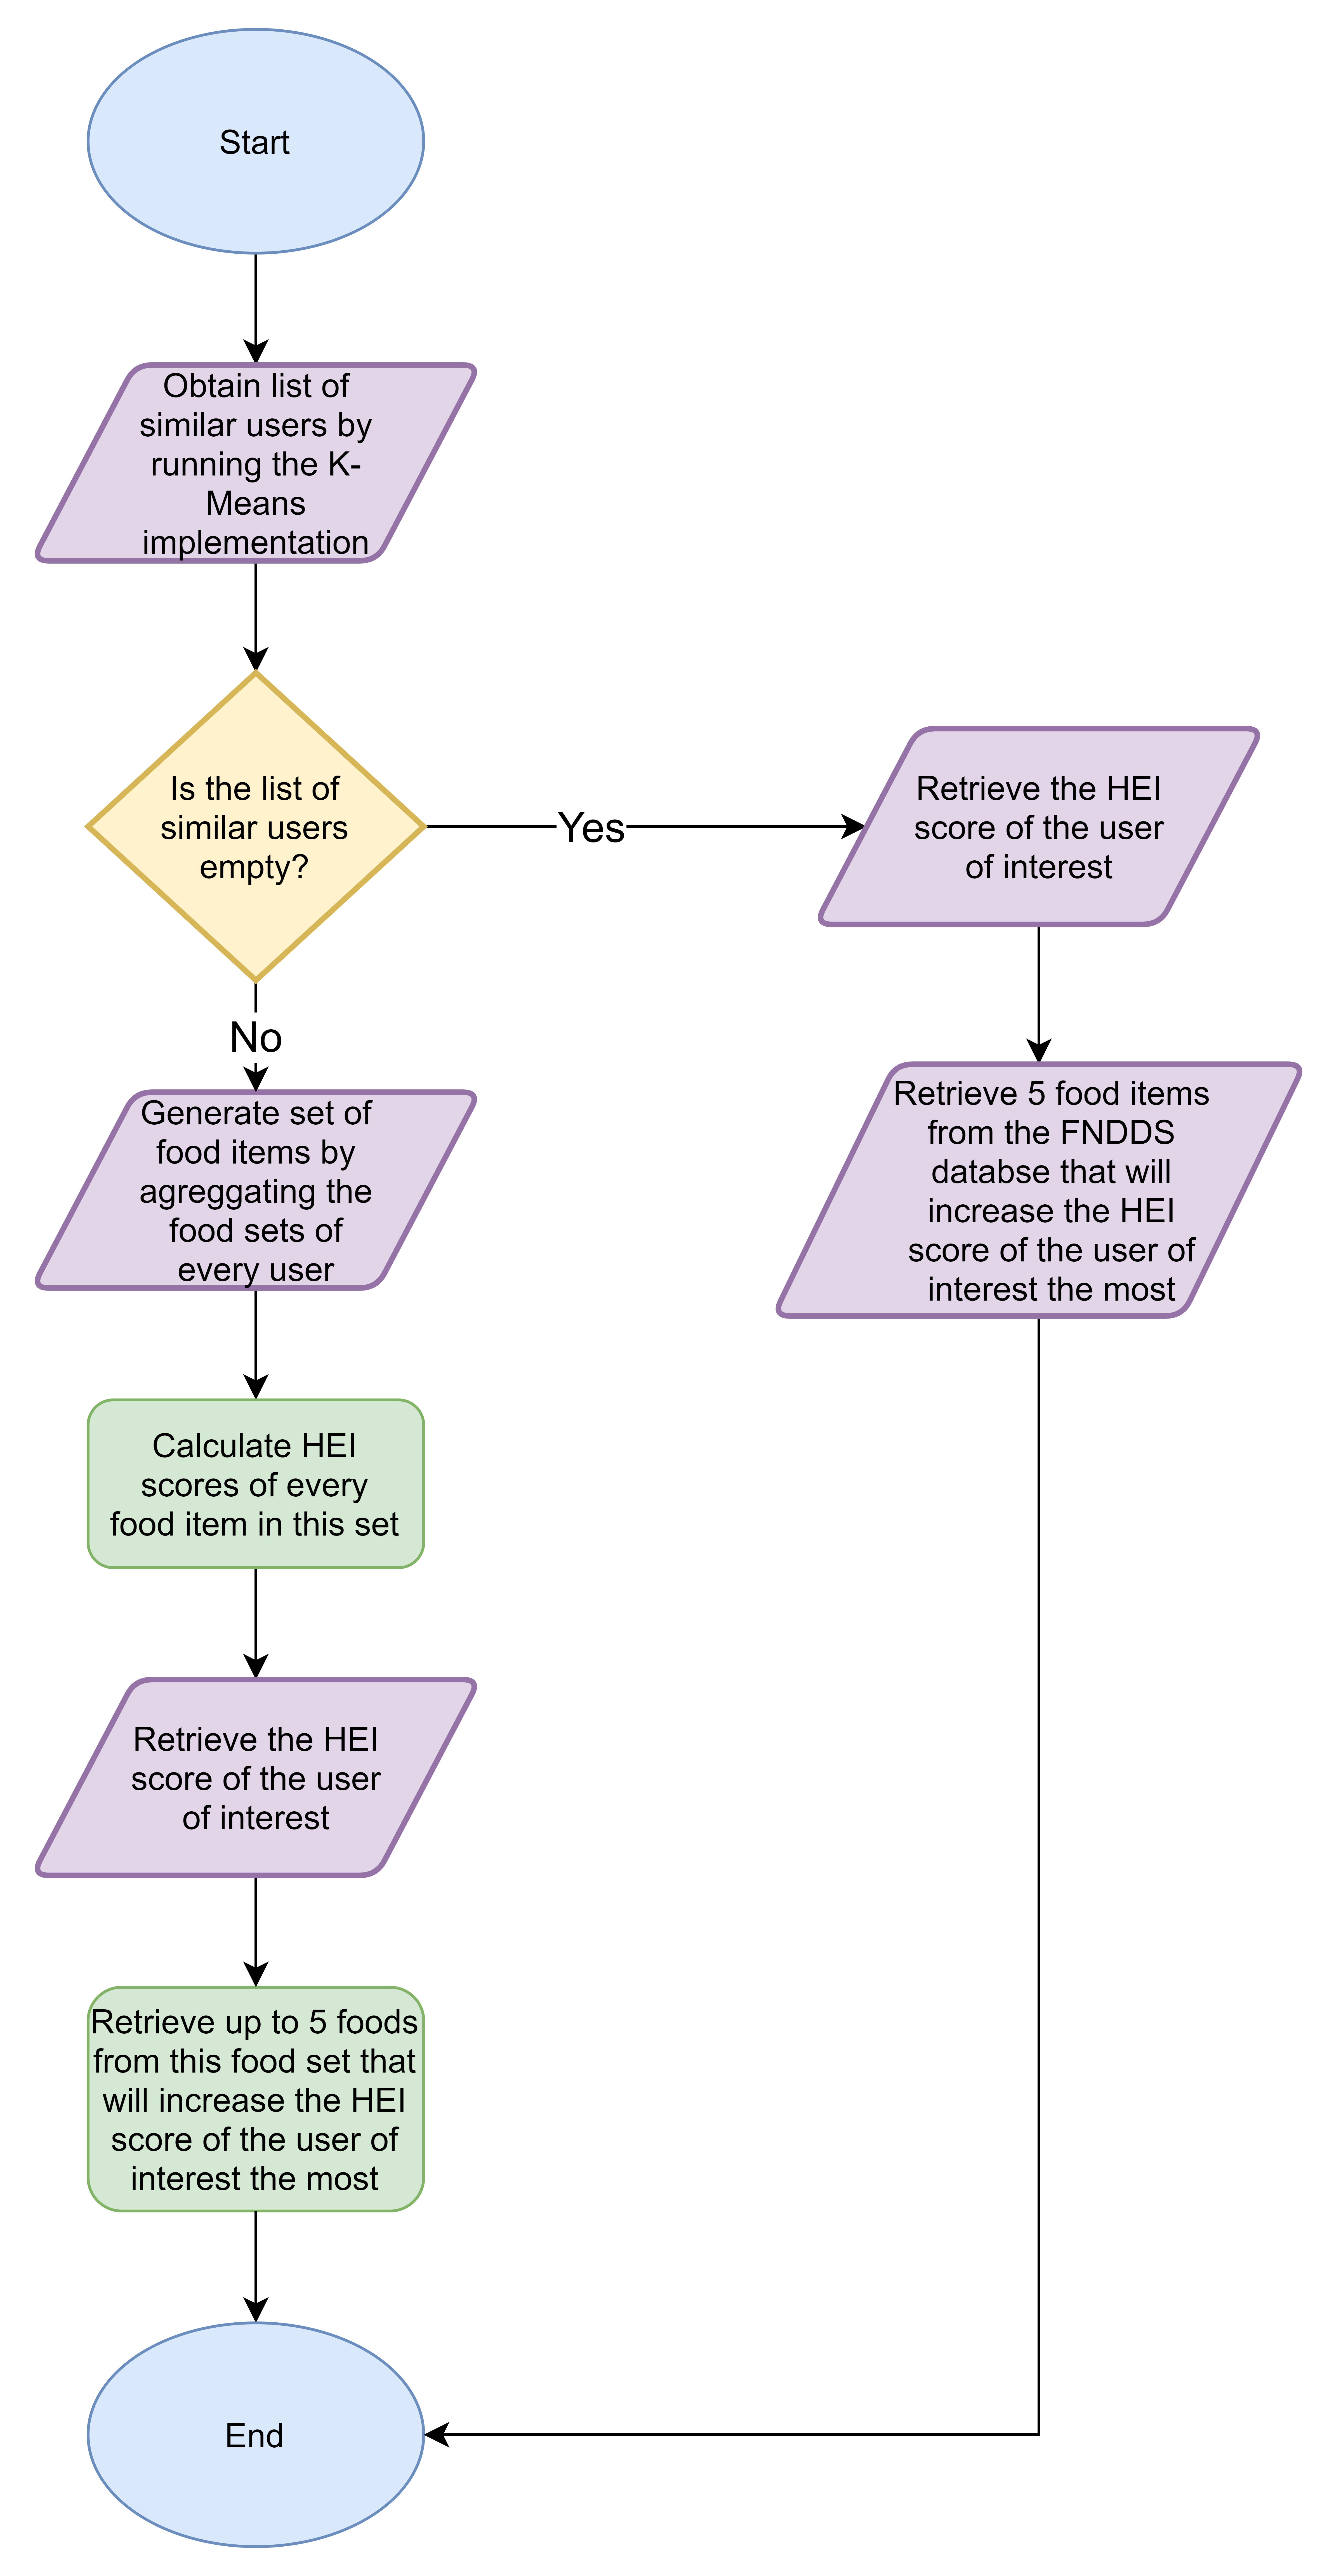
\includegraphics[width = 6cm]{collaborative_filtering.png}
    \caption{Steps in the Recommender System}
    \label{fig:collaborative_filtering}
\end{figure}

\subsubsection{Filtering Set of Foods User is Likely to Enjoy}
A problem I ran into during the implementation process, was the sheer size of the generated food set, which slowed down the response time significantly. A straightforward solution was to limit the number of similar users considered in the program. K-Means implementation was modified to return at most 3 users from the same cluster as the user of interest. 3 closest users were picked. This greatly sped up the process. 

\bigskip
\noindent Two approaches came to mind about how to filter out unhealthy foods from the set of foods the user of interest is likely to enjoy. The approach that I implemented was to simply return 5 food items that increased the users average HEI score the most. This is determined by the average HEI score of the individual food item.

\bigskip
\noindent Potentially a better way to approach this would be to look to balance out the diet of the user of interest. This could be achieved by weighting the components. The degree to which the food item helps balance the HEI score can be determined using the following formula, where foodHEI\textsubscript{i} represents the value of an HEI component for the food item, and similarly userHEI\textsubscript{j} represents the value of an HEI component for the user: 

\begin{align*}
    usefulness &= \frac{1}{13} \sum_{i=1}^{13} foodHEI_{i} * w(i)
\end{align*}

\begin{align*}
    w(i) = \frac{\sum_{j=1}^{13} userHEI_{j}}{userHEI_{j}}
\end{align*}

\bigskip
\noindent The proposed weighting system may not be optimal. Finding the optimal weighting function would require further analysis, which is why I chose the simpler of the two proposed methods.

\section{Evaluation}
\subsection{Evaluation of the HEI Score Estimates}
Majority of the food diary entries in the MyFitnessPal dataset \cite{diet_success_predictions} include information on the sodium content of the food items, which happens to be on the HEI components. Due to time constraints, it was infeasible to evaluate the outcome of the project by manually computing the HEI score of a set of foods and comparing that to the output of the HEI estimating program. A more practical approach would be to compare the estimated sodium content of a set of foods produced by the program, to the actual sodium content, derived directly from the dataset. 

\bigskip 
\noindent I am assuming that the accuracy of the sodium content estimate is the same, or similar to the accuracy of the estimates of the other HEI components.

\subsubsection{Implementing Evaluation Program}
A modified version of the HEI scoring application was made. In order to speed up the process, any unnecessary steps involving any calculations other than those relevant to sodium were removed. The end result was a program that returns the total estimated and actual values for the sodium content of a set of foods. 

\bigskip
\noindent Comparing actual and estimated HEI scores for sodium would be incorrect. A set of foods with less than 1.1g of sodium per 1000 kcal would be given the maximum 10 points. Similarly, a set of foods exceeding 2.0g of sodium per 1000 kcal would be given the minimum score of 0. Therefore different food sets with sodium contents above or below the 1.1-2.0g of sodium per 1000kcal would have identical scores, which would not give any insight on the accuracy of the estimate. 

\subsubsection{HEI Score Evaluation Results}
Due to the size of the dataset, I deemed random sampling to be the most suitable approach. The 'DateFoodSetNut' table contains the set of foods consumed, sorted by user and date. 100 such sets were randomly picked and used as input for the evaluation program. The average percentage error turned out to be 2340\%. 

\bigskip
\noindent I believe that there are multiple causes for such a high average percentage error. One such cause being that the HEI score was estimated rather than calculated. The FNDDS and FPED databases were of great use, but unfortunately, they were very small, containing only 9000 food items. The MyFitnessPal dataset \cite{diet_success_predictions} contains food items that are not in the databases, so the food item with the highest string similarity in the databases was used instead. HEI could be calculated directly by looking up the ingredients of the food items and their amounts. This could be a standalone project. Additionally, the portion size was estimated using calorie content, as it was not available in the dataset. 

\bigskip
\noindent Another such cause is my string matching implementation. I would have liked to experiment with EM clustering with GMM, as well as with text preprocessing techniques, but unfortunately, I was unable to do so in the given time frame.

\bigskip
\noindent I believe that another cause for such inaccuracy to be the limiting resources. Both the databases and the dataset are relatively small. Additionally, the dataset was missing important information, such as portion size. My recommender system used an implicit collaborative filtering technique, had the dataset included food ratings, explicit collaborative filtering techniques could have been used instead. This would have allowed me to make fewer assumptions and result in more accurate user models. In turn, that would have resulted in better predictions. 

\subsection{Evaluation of the Recommender System}
\subsubsection{Using My Personal Input}
A simple approach to the evaluation of the recommender system would be to supply the food I eat as input and comment on whether I like the recommended food items or not. Having retrieved nutritional information from the packaging, I supplied my typical daily diet as input, see Table \ref{table:my_typical_input}.

\begin{table}[h]
\centering
\hspace*{-0.25cm}
\begin{tabular}{||m{2cm}|m{2cm}|m{5cm}||}
\hline
    Calories (kcal) & Sodium (mg) &  Food Description\\ 
    \hline
    750 & 2180 & BBQ Chicken Pizza\\
    \hline
    244 & 100 & Magnum Chocolate Ice Cream\\
    \hline
    840 & 1150 & Beef Mince\\
    \hline
    230 & 3195 & Chilli con carne sauce\\
    \hline
    894 & 2460 & Doritos\\
    \hline 
    2 & 200 & Monster Energy Drink\\
\hline
\end{tabular}
\caption{My Typical Daily Diet}
\label{table:my_typical_input}
\end{table}

\noindent Figure \ref{fig:my_input_results} show the result that the application displays. I believe that the HEI score estimate does capture the overall trend, and evaluating the estimate gave a percentage error of just 47\%. The recommender system suggested apple chips, eggs, sesame seeds, falafel, and chicken or turkey salad. I really like chicken and eggs, these two suggestions are quite good, eggs being a staple food in my diet. I do enjoy apples, but I do not eat them frequently, hence this is the best suggestion, as I clearly do not eat enough fruits and vegetables. On the other hand, neither sesame seeds nor falafel are the kinds of foods I think I would enjoy. 3 out of the 5 suggestions are acceptable and I would consider to be successful recommendations.

\begin{figure}[h]
\centering
\hspace*{-1cm} 
\begin{subfigure}{.5\textwidth}
  \centering
  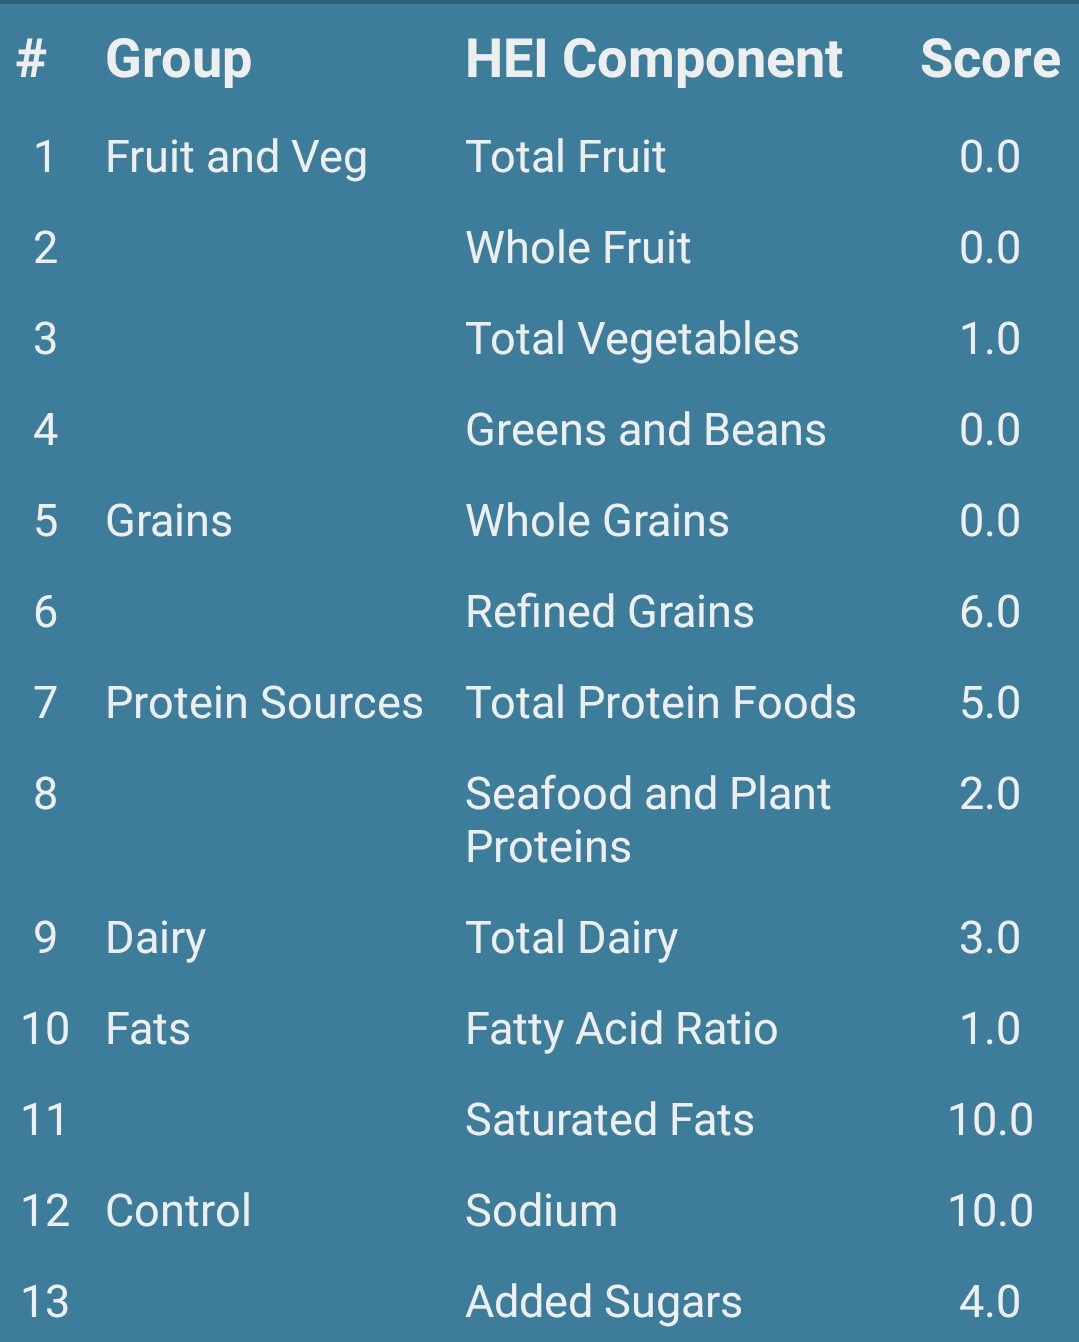
\includegraphics[height = 5cm]{my_input_hei_table.jpg}
  \caption{HEI Score in a Radar Graph}
  \label{fig:my_input_hei_radar_graph}
\end{subfigure}%
\begin{subfigure}{.4\textwidth}
  \centering
  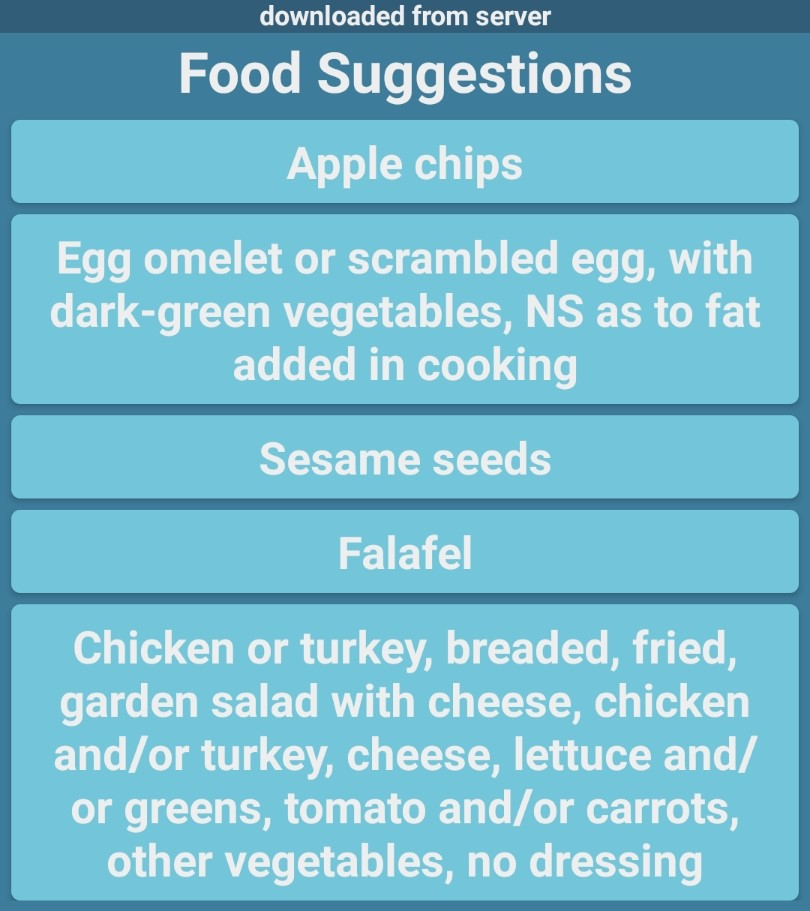
\includegraphics[height = 5cm]{my_input_recommendations.jpg}
  \caption{Recommendations Received}
  \label{fig:my_input_recommendations}
\end{subfigure}
\begin{subfigure}{\textwidth}
  \centering
  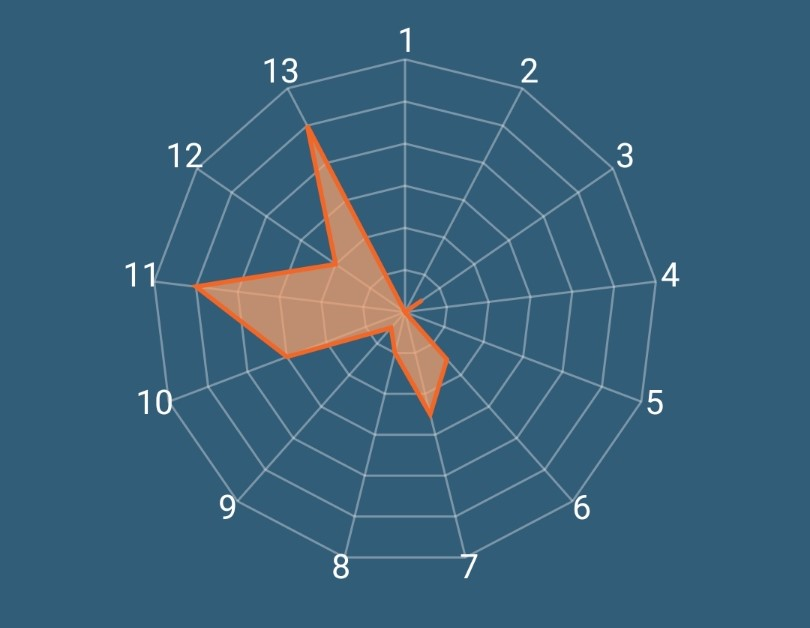
\includegraphics[height = 6cm]{my_input_hei_radar_graph.jpg}
  \caption{HEI Score in a Table}
  \label{fig:my_input_hei_table}
\end{subfigure}
\caption{Screenshots of the Application Upon Providing My Daily Food Intake}
\label{fig:my_input_results}
\end{figure}

\subsubsection{Using an Input from Dataset}
I decided to run the recommender system using the input from a user in the dataset. I used user with user\_id=1, and date='2014-09-21'. The recommendations produced were: 

\begin{enumerate}
    \item Egg omelet or scrambled egg, with dark-green vegetables, NS as to fat added in cooking.
    \item Falafel.
    \item Pesto sauce.
    \item Fish curry.
    \item White beans, dry, cooked, NS as to fat added in cooking.
\end{enumerate}

\bigskip
\noindent Although it would be impossible to verify whether or not that user would like the recommended food items, an inspection of that user's food set will give a vague idea. Records show that user consumed food items with the following descriptions:

\begin{itemize}
    \item \textit{'Eggs - Poached (whole egg), 2 large'.}
    \item \textit{'Eurest - Curry Chicken, 2 serving(s)'}
    \item \textit{'Morrisons - Chicken & Basil Pesto Pasta, 200 g Pack'}
    \item \textit{'Mao - Seafood Laksa, 1 bowl'}
    \item \textit{'Beans Green - Boiled, 50 g'}
    \item \textit{'Heinz - Baked Beans - 201, 220 g'}
    \item \textit{'Dim Sum - Shrimp Dumplings, 6 pc'}
\end{itemize}

\bigskip
\noindent I think that recommendation 1 is reasonable because the user consumed poached eggs and green beans in the past. I also believe recommendation 3 to be reasonable, as the user consumed chicken and basil pesto pasta. Recommendation 5 is a healthier alternative to baked beans, and thus an improvement. I think that recommendations 1, 3, and 5 are thus very logical.

\bigskip
\noindent It is difficult to say whether or not the user would like recommendation 4. That user has previously consumed seafood products, such as shrimp dumplings and seafood laksa, and chicken curry, but it is impossible to comment on another person's subjective liking. However, I do believe it is reasonable to assume that fish curry is a sensible suggestion, given the record.

\bigskip
\noindent Overall, 4 out of the 5 suggestions produced by the recommender system are very reasonable. 

\section{Conclusion}
In conclusion, I successfully implemented a cloud-based application that estimates the HEI score of a user based on the food input they provided. The application also uses a machine-learning algorithm to produce useful suggestions on what enjoyable foods the user could eat to maximise their HEI score. 

%%TC:ignore
\newpage
\begin{thebibliography}{9}
\bibitem{FNDDS}
Food and Nutrient Database for Dietary Studies [online] Available at: \textit{https://www.ars.usda.gov/northeast-area/beltsville-md-bhnrc/beltsville-human-nutrition-research-center/food-surveys-research-group/docs/fndds-download-databases/}
\bibitem{FPED}
Food Patterns Equivalents Database [online] Available at: 
\textit{https://www.ars.usda.gov/northeast-area/beltsville-md-bhnrc/beltsville-human-nutrition-research-center/food-surveys-research-group/docs/fped-data-tables/}
\bibitem{tempted_brain} 
Berridge, K.C., Ho, C.-Y., Richard, J.M. and DiFeliceantonio, A.G. (2010). 
\textit{The tempted brain eats: Pleasure and desire circuits in obesity and eating disorders. Brain Research, 1350, pp.43–64.}. 
\bibitem{craving_time}
Reichenberger, J., Richard, A., Smyth, J.M., Fischer, D., Pollatos, O. and Blechert, J. (2018).
\textit{It’s craving time: time of day effects on momentary hunger and food craving in daily life. Nutrition, 55–56, pp.15–20.}
\bibitem{ml_enterprises}
Lee, I. and Shin, Y.J. (2019). \textit{Machine learning for enterprises: Applications, algorithm selection, and challenges. Business Horizons.}
\bibitem{passive_mvc}
Sokolova, K., Lemercier, M. and Garcia, L. (2013). \textit{Android Passive MVC: a Novel Architecture Model  for Android Application Development.PATTERNS 2013 : The Fifth International Conferences on Pervasive Patterns and Applications.}
\bibitem{satiety_satiation}
Campbell, C.L., Wagoner, T.B. and Foegeding, E.A. (2017). \textit{Designing foods for satiety: The roles of food structure and oral processing in satiation and satiety. Food Structure, 13, pp.1–12.}
\bibitem{weight_expenditure}
Fonseca, D.C., Sala, P., de Azevedo Muner Ferreira, B., Reis, J., Torrinhas, R.S., Bendavid, I. and Linetzky Waitzberg, D. (2018). \textit{Body weight control and energy expenditure. Clinical Nutrition Experimental, 20, pp.55–59.}
\bibitem{binge_freq}
Zendegui, E.A., West, J.A. and Zandberg, L.J. (2014). \textit{Binge eating frequency and regular eating adherence: The role of eating pattern in cognitive behavioral guided self-help. Eating Behaviors, 15(2), pp.241–243.}
\bibitem{hei_2015}
Krebs-Smith, S.M., Pannucci, T.E., Subar, A.F., Kirkpatrick, S.I., Lerman, J.L., Tooze, J.A., Wilson, M.M. and Reedy, J. (2018). \textit{Update of the Healthy Eating Index: HEI-2015. Journal of the Academy of Nutrition and Dietetics, 118(9), pp.1591–1602.}
\bibitem{micro_quality}
Gardner, C.D., Kim, S., Bersamin, A., Dopler-Nelson, M., Otten, J., Oelrich, B. and Cherin, R. (2010). \textit{Micronutrient quality of weight-loss diets that focus on macronutrients: results from the A TO Z study. The American Journal of Clinical Nutrition, 92(2), pp.304–312.}
\bibitem{cloud_computing}
Dillon, T., Wu, C. and Chang, E. (2010). \textit{Cloud Computing: Issues and Challenges.}
\bibitem{craving_sweets}
Christensen, L. (2007). \textit{Craving for sweet carbohydrate and fat-rich foods - possible triggers and impact on nutritional intake. Nutrition Bulletin, 32(s1), pp.43–51.}
\bibitem{food_label}
Europa.eu. (2011). EUR-Lex - 32011R1169 - EN - EUR-Lex. [online] Available at: \textit{https://eur-lex.europa.eu/legal-content/EN/ALL/?uri=CELEX\%3A32011R1169} [Accessed 27 Nov. 2019].
\bibitem{android_fundamentals}
Android Developers. (2019). Application Fundamentals  |  Android Developers. [online] Available at: \textit{https://developer.android.com/guide/components/fundamentals} [Accessed 1 Dec. 2019].
\bibitem{android_app_architecture}
Android Developers. (2020). Guide to App Architecture | Android Developers. [online] Available at: \textit{https://developer.android.com/jetpack/docs/guide#overview} [Accessed 5 May. 2020]
\bibitem{android_view}
Android Developers. (2020). View | Android Developers. [online] Available at: \textit{https://developer.android.com/reference/android/view/View} [Accessed 5 May. 2020]
\bibitem{android_fragment}
Android Developers. (2020). Fragments | Android Developers. [online] Available at: 
\textit{https://developer.android.com/guide/components/fragments} [Accessed 5 May. 2020]
\bibitem{android_view_model}
Android Developers. (2020). ViewModel | Android Developers. [online] Available at: 
\textit{https://developer.android.com/reference/androidx/lifecycle/ViewModel} [Accessed 5 May. 2020]
\bibitem{android_live_data}
Android Developers. (2020). LiveData | Android Developers. [online] Available at: 
\textit{https://developer.android.com/topic/libraries/architecture/livedata} [Accessed 5 May. 2020]
\bibitem{android_room}
Android Developers. (2020). Room | Android Developers. [online] Available at: 
\textit{https://developer.android.com/topic/libraries/architecture/room} [Acceesed 5 May. 2020]
\bibitem{mvvm}
Gossman, J. (2005) Introduction to Model/View/ViewModel pattern for building WPF apps. [online] Available at: \textit{https://blogs.msdn.microsoft.com/johngossman/2005/10/08/introduction-to-modelviewviewmodel-pattern-for-building-wpf-apps/} [Accessed 5 May. 2020]
\bibitem{diet_success_predictions}
Ingmar Weber and Palakorn Achananuparp. (2016). \textit{Insights from Machine-Learned Diet Success Prediction. In Proceedings of Pacific Symposium on Biocomputing (PSB).}
\bibitem{library_mpandroidchart}
Jahoda, P. (2020) MPAndroidChart  \textit{(API version 3.1.0) https://github.com/PhilJay/MPAndroidChart}
\bibitem{retrofit}
Square Open Source (2020) Retrofit \textit{(API version 2.7.1) https://square.github.io/retrofit/}
\bibitem{apache_opennlp}
Apache Software Foundation (2020) Apache OpenNLP \textit{(API version 1.7.2) https://opennlp.apache.org/}
\bibitem{docker}
Docker, Inc. (2020) Docker \textit{(Version 19.03) https://www.docker.com/}
\bibitem{intellij}
JetBrains s.r.o. (2020) IntelliJ IDEA Ultimate \textit{(Version 2020.1) https://www.jetbrains.com/idea/}
\bibitem{apache_tomcat}
Apache Software Foundation (2020) Apache Tomcat \textit{(Version 9.0.34) http://tomcat.apache.org/}
\bibitem{apache_tomcat_web_xml}
Apache Software Foundation (2020) Apache Tomcat [online] Available at: \textit{http://tomcat.apache.org/tomcat-7.0-doc/appdev/web.xml.txt} [Accessed 8 May. 2020]
\bibitem{fuzzy_wuzzy}
Cohen, A. et al. (2020) FuzzyWuzzy Java Implementation \textit{(Version 1.3.0) https://github.com/xdrop/fuzzywuzzy} 
\bibitem{levenshtein_distance}
Levenshtein, V. I, (1966) \textit{Binary Codes Capable of Correcting Deletions, Insertions and Reversals, Soviet Physics Doklady, Vol. 10, p.707}
\bibitem{jaccard}
Jaccard, P. (1901) \textit{Étude comparative de la distribution florale dans une portion des Alpes et des Jura, Bulletin de la Société vaudoise des sciences naturelles, 37: 547–579}
\bibitem{string_similarity_ontology}
Cheatham, M. et. al. (2013) \textit{String Similarity Metrics for Ontology Alignment, The Semantic Web – ISWC 2013. ISWC 2013. Lecture Notes in Computer Science, vol 8219. Springer, Berlin, Heidelberg}
\bibitem{recommender_systems_handbook}
Ricci, F. et. al. (2011) \textit{Introduction to recommender systems handbook. In Recommender systems handbook}
\bibitem{wagner_fischer}
R. A. Wagner and M. J. Fischer (1974) \textit{The string-to-string correction problem, Journal of the ACM, Vol. 21, No. 1, pp. 168-173}
Ricci, F. et. al. (2011) \textit{Introduction to Recommender Systems Handbook. Recommender Systems Handbook, 1, pp.1-35.}
\bibitem{mongue_elkan}
Jimenez, S. et. al. (2009) \textit{Generalized Mongue-Elkan Method for
Approximate Text String Comparison, Computational Linguistics and Intelligent Text Processing, 10th edition, pp. 560-570}
\bibitem{k_means}
Seif, G. (2018) The 5 Clustering Algorithms Data Scientists Need to Know. [online] Available at: \textit{https://towardsdatascience.com/the-5-clustering-algorithms-data-scientists-need-to-know-a36d136ef68} [Accessed 7 May. 2020]
\bibitem{gmm}
Lingling, N. et. al. (2020) \textit{Streamflow forecasting using extreme gradient boosting model coupled with Gaussian mixture model, Journal of Hydrology, Volume 586}
\bibitem{expectation_maximisation}
Dempster, A. P. et. al. (1977) \textit{Maximum Likelihood from Incomplete Data via the EM Algorithm, Journal of the Royal Statistical Society. Series B (Methodological) Vol. 39, No. 1, pp. 1-38}
\bibitem{http}
Fielding, R. et. al. (1999) Hypertext Transfer Protocol. [online] Available at: \textit{https://tools.ietf.org/html/rfc2616} [Accessed 7 May. 2020]
\bibitem{getting_healthy}
Mitchell, J. et. al. (2015) \textit{\#Gettinghealthy: The perceived influence of social media on young adult health behaviors, Computers in Human Behavior, Volume 45 pp.151-157}
\end{thebibliography}

\newpage
\begin{appendicies}
\section{Appendix A}
\begin{table}[!htbp]
\centering
\hspace*{-0.5cm}
\begin{tabular}{||m{6cm}|m{6cm}||}
    \hline
    UC1 & Sign In\\
    \hline
    Description & Signing in to the application upon application launch\\
    \hline
    Actors & User, Server\\
    \hline
    & Starts when: user launches the application. \newline
    Ends when: user successfully logs into the application or the application shows an error message.\\
    \hline
    \multirow{4}{\hsize}{Basic Flow} 
                                    & 1.) User launches the application\\
                                    & 2.) User  enters  correct  credentials  for an existing account\\ 
                                    & 3.) User clicks the login button\\
                                    & 4.) Authentication successful - user is taken to meal logger screen\\
    \hline
    Exception Flow & Failure to connect to server to authenticate user, incorrect credentials and nonexistent credentials could cause failure at step 4, at which point the user is notified by a dialog box with an error message\\
\hline
\end{tabular}
\caption{Use Case 1}
\label{table:UC1}
\end{table}
\begin{table}[!htbp]
\centering
\hspace*{-0.5cm}
\begin{tabular}{||m{6cm}|m{6cm}||}
    \hline
    UC2 & Sign Up\\
    \hline
    Description & Creating an account to use the application\\
    \hline
    Actors & User, Server\\
    \hline
    & Starts when: user clicks the “sign up” button at the login screen \newline
    Ends when: user account successfully created\\
    \hline
    \multirow{7}{\hsize}{Basic Flow} 
                                    & 1.) User clicks the “sign up” button at the login screen\\
                                    & 2.) User is taken to sign up page\\ 
                                    & 3.) User enters their email, password and unique username into correct text fields\\
                                    & 4.) User is sent authentication code to the provided email address\\
                                    & 5.) The user is taken to authentication code input screen\\
                                    & 6.) User verifies their email by entering the authentication code\\
                                    & 7.) The user is taken to the home screen\\
    \hline
    Alternate Flow & The user may click “cancel” button at any point during steps 2-6\\
    \hline 
    Exception Flow & The user may not receive authentication email, the authentication code inputted at step 6 could be incorrect or email verification could fail due to connection loss to server. The  user is notified by a dialog box with error message\\
\hline
\end{tabular}
\caption{Use Case 2}
\label{table:UC2}
\end{table}

\begin{table}[!htbp]
\centering
\hspace*{-0.5cm}
\begin{tabular}{||m{6cm}|m{6cm}||}
    \hline
    UC3 & Log a Meal\\
    \hline
    Description & User logs a meal\\
    \hline
    Actors & User\\
    \hline
    & Starts when: user is at the meal logger screen \newline
    Ends when: meal is successfully logged\\
    \hline
    \multirow{6}{\hsize}{Basic Flow} 
                                    & 1.) User navigates to meal logger screen in the application\\
                                    & 2.) User clicks “add meal” button\\ 
                                    & 3.) User enters foods consumed\\
                                    & 4.) User enters total calories, proteins, carbs and fats consumed\\
                                    & 5.) User clicks “save” button\\
                                    & 6.) Meal is logged as a JSON object\\
    \hline
    Alternate Flow & The user may click “cancel” button at any point during steps 3 and 4\\
    \hline 
    Exception Flow & The application may not save the logged meal, for example if there isn’t enough local storage on the mobile device. The user is notified by a dialog box with an error message\\
\hline
\end{tabular}
\caption{Use Case 3}
\label{table:UC3}
\end{table}


\begin{table}[!htbp]
\centering
\hspace*{-0.5cm}
\begin{tabular}{||m{6cm}|m{6cm}||}
    \hline
    UC4 & Delete Logged Meal\\
    \hline
    Description & Delete an erroneous meal\\
    \hline
    Actors & User\\
    \hline
    & Starts when: the user is at the meal logger screen and has identified a logged meal they wish to delete \newline
    Ends when: the erroneous meal is deleted\\
    \hline
    \multirow{6}{\hsize}{Basic Flow} 
                                    & 1.) User navigates to meal logger screen\\
                                    & 2.) User selects the desired meal\\ 
                                    & 3.) User clicks “delete” button\\
                                    & 4.) User is presented with dialog box asking for confirmation to delete the meal\\
                                    & 5.) User clicks “OK” button \\
                                    & 6.) Meal is deleted from meal logger\\
    \hline
    Alternate Flow & The user may click “cancel” at step 4\\
    \hline 
    Exception Flow & The application may not delete the meal. This could arise if information is stored in the cloud and across multiple servers\\
\hline
\end{tabular}
\caption{Use Case 4}
\label{table:UC4}
\end{table}

\begin{table}[!htbp]
\centering
\hspace*{-0.5cm}
\begin{tabular}{||m{6cm}|m{6cm}||}
    \hline
    UC5 & Navigate to Desired Screen\\
    \hline
    Description & Navigating between the meal logger screen and the summary screen\\
    \hline
    Actors & User\\
    \hline
    & Starts when: user is at the meal logger screen \newline
    Ends when: user is at the summary screen\\
    \hline
    \multirow{5}{\hsize}{Basic Flow} 
                                    & 1.) User is at the meal logger screen\\
                                    & 2.) User clicks the side toolbar button\\ 
                                    & 3.) Side toolbar appears on the edge of the screen\\
                                    & 4.) User clicks “Summary” button\\
                                    & 5.) User is taken to summary screen\\
    \hline
    Alternate Flow & The user may click any other option available in the toolbar or go from summary screen to meal logger screen\\
    \hline 
    Exception Flow & The summary screen may not load due to a bug in the code or a glitch in the operating system of the mobile device the app is run on\\
\hline
\end{tabular}
\caption{Use Case 5}
\label{table:UC5}
\end{table}


\begin{table}[!htbp]
\centering
\hspace*{-0.5cm}
\begin{tabular}{||m{6cm}|m{6cm}||}
    \hline
    UC6 & Log Out\\
    \hline
    Description & Logging out of the application\\
    \hline
    Actors & User\\
    \hline
    & Starts when: a user is logged into the application \newline
    Ends when: the application is at the login page\\
    \hline
    \multirow{7}{\hsize}{Basic Flow} 
                                    & 1.) User is logged into the application\\
                                    & 2.) User clicks the side toolbar button\\
                                    & 3.) Side toolbar appears on the edge of the screen\\
                                    & 4.) User clicks the “logout” button at the bottom of the toolbar\\
                                    & 5.) User is presented with dialog box asking for confirmation to logout\\
                                    & 6.) User clicks “OK” button\\
                                    & 7.) Application displays the login page\\
    \hline
    Alternate Flow & The user may click “cancel” button during step 5\\
    \hline 
    Exception Flow & The application may not logout the user due to a bug in the code or a glitch in the operating system of the mobile device the app is run on\\
\hline
\end{tabular}
\caption{Use Case 6}
\label{table:UC6}
\end{table}

\begin{table}[!htbp]
\centering
\hspace*{-0.5cm}
\begin{tabular}{||m{6cm}|m{6cm}||}
    \hline
    UC7 & Upload Logged Meals to Server\\
    \hline
    Description & Logged meals are uploaded to server for analysis\\
    \hline
    Actors & Server\\
    \hline
    & Starts when: server requests logged meals or user requests HEI calculation \newline
    Ends when: meals are saved in server storage\\
    \hline
    \multirow{4}{\hsize}{Basic Flow} 
                                    & 1.) Server requests logged meals\\
                                    & 2.) The logged meals are parsed as a single JSON object\\
                                    & 3.) The JSON object is sent to the server\\
                                    & 4.) The server saves the JSON object in its storage\\
    \hline
    Exception Flow & The server may not receive the logged meal or receive corrupted log, for example if the internet connection has been disrupted during the process. For this process, acknowledgements must be used\\
\hline
\end{tabular}
\caption{Use Case 7}
\label{table:UC7}
\end{table}

\begin{table}[!htbp]
\centering
\hspace*{-0.5cm}
\begin{tabular}{||m{6cm}|m{6cm}||}
    \hline
    UC8 & Calculate HEI Score\\
    \hline
    Description & Calculating HEI score based on the meals logged by the user\\
    \hline
    Actors & Server\\
    \hline
    & Starts when: all food items logged by a user have been mapped to food items in the FNDDS\newline
    Ends when: HEI score is calculated\\
    \hline
    \multirow{3}{\hsize}{Basic Flow} 
                                    & 1.) Once all food items logged by a user have been mapped to food items in the FNDDS, the ratio multiplier is calculated by dividing user inputted calories by calories in the FNDSS database.\\
                                    & 2.) The amounts of all necessary food groups are looked up for the food item in the Food Patterns Equivalents Database (FPED) and multiplied by the ratio multiplier\\
                                    & 3.) The gathered information about the food groups is inputted into the HEI scoring algorithm, which is provided by the United States Department of Agriculture (USDA), outputting the HEI score for that particular user\\
    \hline
    Exception Flow & The server may not receive the logged meal or receive corrupted log, for example if the internet connection has been disrupted during the process. For this process, acknowledgements must be used\\
\hline
\end{tabular}
\caption{Use Case 8}
\label{table:UC8}
\end{table}

\begin{table}[!htbp]
\centering
\hspace*{-0.5cm}
\begin{tabular}{||m{6cm}|m{6cm}||}
    \hline
    UC9 & View Previous Logs\\
    \hline
    Description & View logged meals for previous days\\
    \hline
    Actors & User\\
    \hline
    & Starts when:  the user is at the meal logger screen and wants to view a meal that they previously logged\newline
    Ends when: the previously logged meal is displayed\\
    \hline
    \multirow{6}{\hsize}{Basic Flow} 
                                    & 1.) User is at the meal logger screen\\
                                    & 2.) User clicks “select day” button\\
                                    & 3.) User is presented with calendar widget\\
                                    & 4.) User navigates to the desired date\\
                                    & 5.) User clicks the desired date\\
                                    & 6.) The meal log for that day is loaded\\
    \hline
    Exception Flow & If the user hasn’t logged any meals for the selected day, no information is going to be presented. The user is notified by a dialog box with an error message\\
\hline
\end{tabular}
\caption{Use Case 9}
\label{table:UC9}
\end{table}

\begin{table}[!htbp]
\centering
\hspace*{-0.5cm}
\begin{tabular}{||m{6cm}|m{6cm}||}
    \hline
    UC10 & Starting the Application\\
    \hline
    Description & Loading the application on a mobile device running Android operating system\\
    \hline
    Actors & User\\
    \hline
    & Starts when:  application is downloaded and located on the user’s device\newline
    Ends when: application is loaded\\
    \hline
    \multirow{3}{\hsize}{Basic Flow} 
                                    & 1.) User locates the application on their home screen\\
                                    & 2.) User clicks the application icon\\
                                    & 3.) The application loads up\\
    \hline
    Alternate Flow & The application may not load due to a bug in the code or an error in the operating system of the device\\
\hline
\end{tabular}
\caption{Use Case 10}
\label{table:UC10}
\end{table}

\newpage
\section{Appendix B}
\begin{figure}[h]
    \centering
    \hspace*{-3.5cm}
    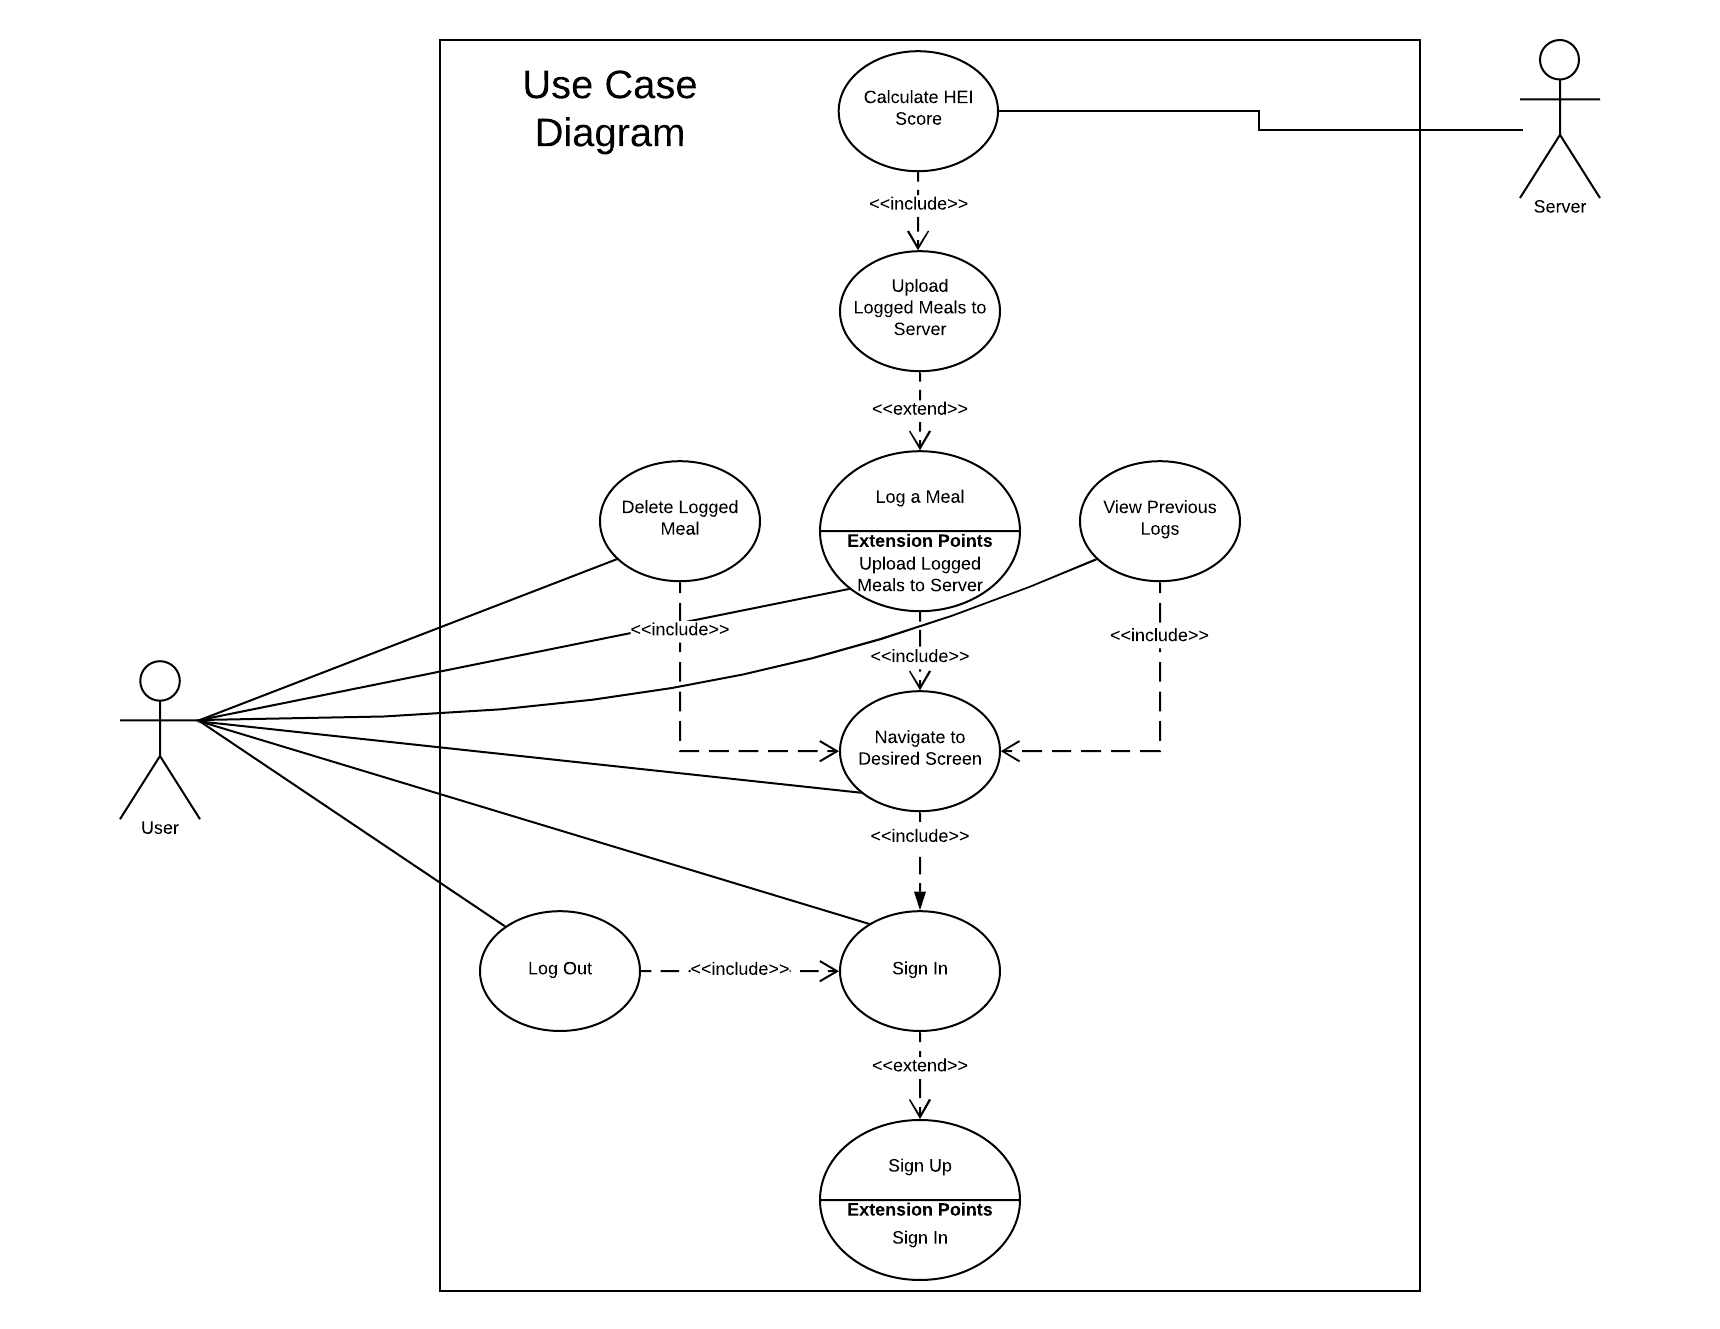
\includegraphics[width = 18cm]{Use case diagram revised.png}
    \caption{Use Case Diagram}
    \label{fig:use_case_diagram}
\end{figure}

\newpage
\section{Appendix C}
\begin{table}[!htbp]
\centering
\hspace*{-2cm}
\begin{tabular}{||m{1cm}|m{9cm}|m{2cm}|m{2cm}||}
    \hline
    Req. ID & Description & Associated Use Case & Req. Number\\
    \hline
    1 & The application should be written for Android  & 10 & 10.1\\
    \hline 
    2 & The application should have internet connection & 7 & 7.1\\
    \hline 
    3 & The application should be a cloud application & 7 & 7.2\\
    \hline 
    4 & The application should securely store user information on the server & 7 & 7.3\\
    \hline 
    5 & The application should have a navigation drawer so that the user can navigate round the application easier & 5 & 5.1\\
    \hline
    6 & The application should have a “Meal Logger” screen where the user can input meals they consumed & 5 & 5.2\\
    \hline
    7 & The application should have a “Summary” screen where the user can view their estimated HEI score & 5 & 5.3\\
    \hline
    8 & The application should allow the user to create a new account upon launch so that they can use the application & 2 & 2.1\\
    \hline 
    9 & The application should allow the user to sign in upon launch so that the user can use the application on multiple different devices & 1 & 1.1\\
    \hline
    10 & The application should only permit successful login with correct credentials & 1 & 1.2\\
    \hline
    11 & The user should be able to log out of the application so that an another user may log in & 6 & 6.1\\
    \hline
    12 & The application should allow the user to log a meal they consumed by providing the names of the food items they consumed and their nutritional values (calories, proteins, carbs and fats) & 3 & 3.1\\
    \hline
    13 & The application should save the logged meals in JSON format & 3 & 3.2\\
    \hline 
    14 & The application should allow the user to view previously logged meals & 9 & 9.1\\
    \hline
    15 & The application should allow the user to delete previous meal entries so that the data input for calculating the HEI score is more representative & 4 & 4.1\\
    \hline
    16 & The application should calculate an estimate of the user’s HEI score (calculations are carried out on the server) & 8 & 8.1\\ 
    \hline 
    17 & The application should recalculate the estimate of the user’s HEI score if the user deleted old entries or added new entries & 8 & 8.2\\
    \hline 
    18 & The application should display the estimated HEI score in a radar graph on the “Summary” screen & 8 & 8.3\\
\hline
\end{tabular}
\caption{Requirements}
\label{table:requirements}
\end{table}


\begin{sidewaysfigure}[h!]
\section{Appendix D}
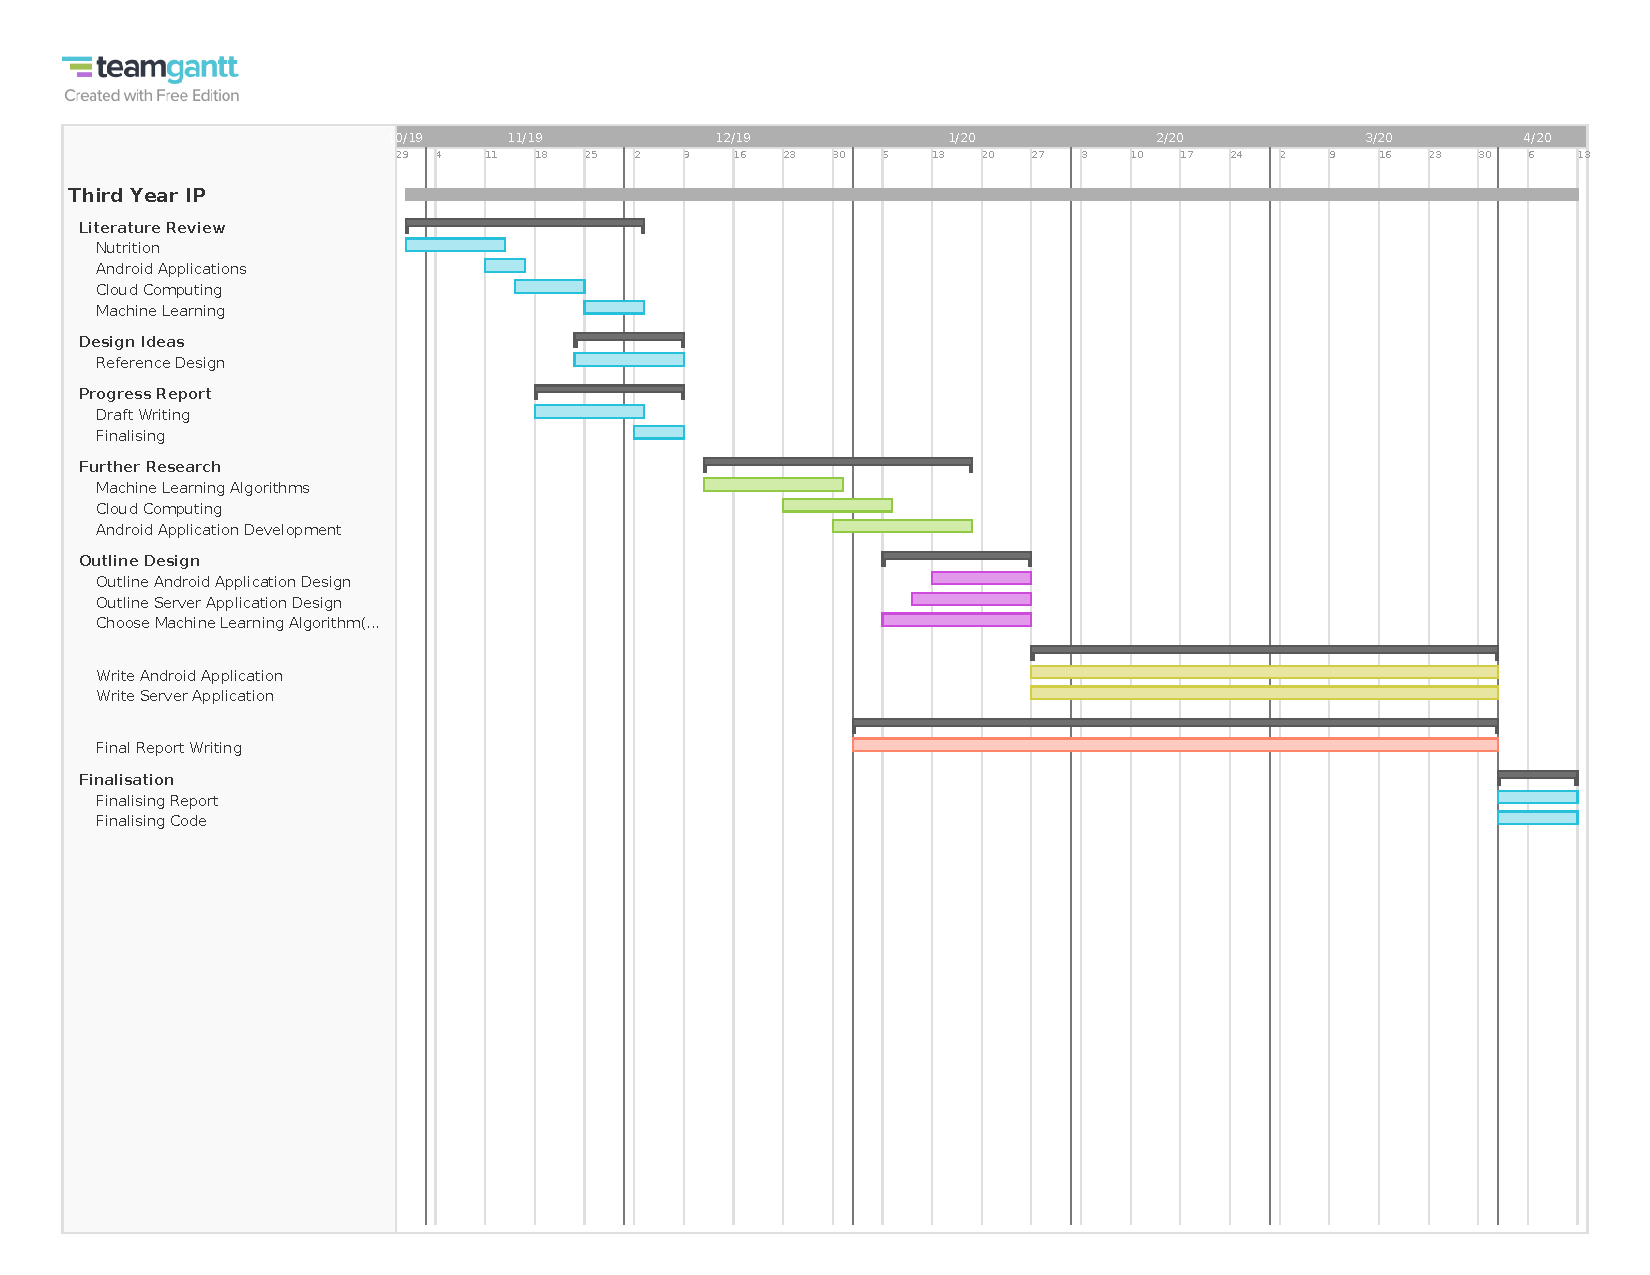
\includegraphics[width=\textwidth]{Third_Year_IP.pdf}
\centering
\caption{Gantt Chart}
\label{fig:gantt_chart}
\end{sidewaysfigure}

\section{Appendix E}
\section*{COVID-19}
Self isolation during lock down has had an impact on my mental health, which resulted in decreased productivity and lack of motivation. Nevertheless, setting targets and milestones helped me implement the project with the core functionality.





\end{appendicies}

%%TC:endignore

\end{document}